% !TeX program = lualatex
% !TeX spellcheck = uk_UA

\documentclass[14pt, a4paper]{extarticle}

% -- Мови та шрифти (згідно з ДСТУ) --
\usepackage{fontspec}
\usepackage[english, ukrainian]{babel}
\usepackage{csquotes}

\setmainfont{Times New Roman}
\setsansfont{Arial}
\setmonofont{Courier New}[Scale=0.85]

% -- Математичні пакети --
\usepackage{amsmath, amssymb, mathtools}

% -- Оптимізація тексту для LuaLaTeX --
\usepackage[protrusion=true, expansion=true]{microtype}
\emergencystretch=3.5em
\hbadness=10000

% -- Параметри сторінки згідно з ДСТУ 3008:2015 --
\usepackage[
    left=30mm,
    right=15mm,
    top=20mm,
    bottom=20mm,
    footskip=10mm,
    headheight=17pt
]{geometry}

% -- Міжрядковий інтервал (еквівалент 1.5 Word) та абзацний відступ --
\linespread{1.3}
\usepackage{indentfirst}
\setlength{\parindent}{1.25cm}
\setlength{\parskip}{0pt}

% -- Колонтитули та нумерація сторінок (вгорі праворуч, без лінійок) --
\usepackage{fancyhdr}
\fancypagestyle{plain}{
    \fancyhf{}
    \rhead{\thepage}
    \renewcommand{\headrulewidth}{0pt}
}
\pagestyle{plain}

% -- Форматування заголовків згідно з ДСТУ 3008:2015 --
\usepackage[explicit]{titlesec}

% Формат розділів (14pt, напівжирний, абзацний відступ 1.25cm)
\titleformat{\section}[block]
{\normalsize\bfseries\raggedright}
{\thesection\ }
{0pt}
{#1}
\titlespacing*{\section}{\parindent}{14pt}{7pt}

% Формат підрозділів
\titleformat{\subsection}[block]
{\normalsize\bfseries\raggedright}
{\thesubsection\ }
{0pt}
{#1}
\titlespacing*{\subsection}{\parindent}{14pt}{7pt}

% -- Списки (компактні, вирівняні за абзацним відступом) --
\usepackage{enumitem}
\setlist{
    nosep,
    leftmargin=*,
    labelindent=\parindent
}
\setlist[itemize]{label=--}

% -- Підписи до рисунків та таблиць згідно з ДСТУ 3008:2015 --
\usepackage{caption}
\DeclareCaptionLabelSeparator{emdash}{ -- }

\captionsetup[figure]{
    labelsep=emdash,
    name={Рисунок},
    justification=centering,
    position=bottom,
    font=normalsize
}

\captionsetup[table]{
    labelsep=emdash,
    name={Таблиця},
    justification=raggedright,
    singlelinecheck=false,
    position=top,
    font=normalsize
}

% -- Таблиці (книжковий стиль, нормальний інтервал) --
\usepackage{booktabs}
\usepackage{tabularx}
\usepackage{multirow}
\newcolumntype{Y}{>{\raggedright\arraybackslash}X}
\renewcommand{\arraystretch}{1.0}

% -- Графіка та гіперпосилання --
\usepackage{graphicx}
\usepackage[hidelinks]{hyperref}

% -- Завантаження модуля обробки таблиць Lua --
\directlua{dofile("tables.lua")}

\begin{document}

% -- Титульна сторінка --
\begin{titlepage}
    \thispagestyle{empty}
    \setlength{\parindent}{0pt}
    
    % -- ШАПКА ДОКУМЕНТА (12pt, напівжирний) --
    \begin{center}
        {\fontsize{12pt}{16pt}\selectfont\bfseries
        МІНІСТЕРСТВО ОСВІТИ І НАУКИ УКРАЇНИ\\[3pt]
        ОДЕСЬКИЙ НАЦІОНАЛЬНИЙ УНІВЕРСИТЕТ ІМЕНІ І.І. МЕЧНИКОВА\\[3pt]
        ФАКУЛЬТЕТ МАТЕМАТИКИ, ФІЗИКИ ТА ІНФОРМАЦІЙНИХ ТЕХНОЛОГІЙ\\[3pt]
        КАФЕДРА ОПТИМАЛЬНОГО КЕРУВАННЯ ТА ЕКОНОМІЧНОЇ КІБЕРНЕТИКИ\par}
    \end{center}

    \vspace{1.5cm}

    % -- НАЗВА РОБОТИ ТА ТЕМА --
    \begin{center}
        {\fontsize{18pt}{22pt}\selectfont\bfseries ЗВІТ\\
        до лабораторної роботи № 6\par}
        \vspace{0.4cm}
        {\fontsize{14pt}{18pt}\selectfont
        з дисципліни «Системи комп’ютерного зору»\par}
        \vspace{0.4cm}
        {\fontsize{16pt}{20pt}\selectfont\bfseries
        на тему:\\[6pt]
        «Оптичний потік і відстеження об’єктів»\par}
    \end{center}

    \vspace{1.5cm}

    % -- ПРАВИЙ БЛОК (Виконавець) --
    \hfill
    \begin{minipage}{0.60\textwidth}
        \raggedright
        {\fontsize{14pt}{19pt}\selectfont
        Виконав:\\[2pt]
        студент 3 курсу групи 1\\[2pt]
        спеціальності F1 «Прикладна математика»\\[2pt]
        Касьянов Ярослав Володимирович
        }
    \end{minipage}

    \vfill

    % -- МІСТО ТА РІК --
    \begin{center}
        {\fontsize{12pt}{14pt}\selectfont\bfseries Одеса -- 2026\par}
    \end{center}
\end{titlepage}

% За ДСТУ титульна сторінка входить у загальну нумерацію як 1-ша, 
% тому наступна сторінка отримує номер 2:
\setcounter{page}{2}


\section{Мета роботи}
Дослідити й порівняти методи розрідженого (\texttt{PyrLK}) і щільного (\texttt{Farneback}) оптичного потоку, віднімання фону \texttt{MOG2} із морфологічним очищенням для підрахунку перетинів контрольної лінії, а також побудувати й кількісно оцінити трекери об'єктів за наявності перекриття з використанням \texttt{cv2.KalmanFilter}.

\section{Вихідні дані}
\begin{itemize}
    \item \textbf{Відео A (\texttt{lab06/data/one\_object.mp4})}: відео зі стаціонарної камери у повнокадровому форматі 4:3 без бічних смуг ($2592 \times 1944$~пк, $30.02$~кадр/с, $656$ кадрів, тривалість $21.85$~с) -- рух одного об'єкта (м'яка іграшка-акула «Блахадж») по світлому паркету з розворотами й багаторазовим перетином горизонтальної лінії.
    \item \textbf{Відео B (\texttt{lab06/data/two\_objects.mp4})}: відео зі стаціонарної камери ($2592 \times 1944$~пк, $29.60$~кадр/с, $354$ кадри, тривалість $11.96$~с) -- рух двох об'єктів («Блахадж» і радіокерована машинка) з епізодом тривалого часткового дотику ($f = 68$--$235$) і повного перекриття машинки за корпусом акули ($f = 273$--$288$).
    \item \textbf{Програмне забезпечення}: Python~3.13, OpenCV (\texttt{cv2}), NumPy, Matplotlib; відеозапис із кодеком \texttt{mp4v}.
\end{itemize}

\section{Теоретичні відомості}
\begin{enumerate}
    \item \textbf{Оптичний потік Лукаса--Канаде (\texttt{PyrLK}) та зворотна перевірка}: з припущення постійності яскравості $I(x,y,t) \approx I(x+\Delta x, y+\Delta y, t+\Delta t)$ випливає лінійне рівняння потоку $I_x u + I_y v + I_t = 0$. Метод Лукаса--Канаде у локальному вікні $W$ розв'язує систему нормальних рівнянь для точок Ши--Томасі ($\min(\lambda_1, \lambda_2) > \lambda_{\min}$), а зворотне відстеження відсіює нестійкі траєкторії за порогом $T_{\text{FB}}$:
    \begin{equation}\label{eq:lk}
    \begin{split}
        \begin{pmatrix} \sum_W I_x^2 & \sum_W I_x I_y \\ \sum_W I_x I_y & \sum_W I_y^2 \end{pmatrix} \begin{pmatrix} u \\ v \end{pmatrix} &= -\begin{pmatrix} \sum_W I_x I_t \\ \sum_W I_y I_t \end{pmatrix}, \\
        e_{\text{FB}} &= \left\| \mathbf{x}_t - \hat{\mathbf{x}}_{t \leftarrow t+1}\!\left(\hat{\mathbf{x}}_{t+1}\right) \right\|_2 \le T_{\text{FB}}.
    \end{split}
    \end{equation}

    \item \textbf{Щільний оптичний потік Фарнебека (\texttt{Farneback})}: окіл кожного пікселя наближується квадратичним поліномом $f(\mathbf{x}) \approx \mathbf{x}^T A \mathbf{x} + \mathbf{b}^T \mathbf{x} + c$; вектор зміщення $\mathbf{d}(\mathbf{x}) = (u, v)^T$ і його полярні координати для HSV-візуалізації визначаються як:
    \begin{equation}\label{eq:farneback}
        A(\mathbf{x})\,\mathbf{d}(\mathbf{x}) = \Delta\mathbf{b}(\mathbf{x}), \quad |\mathbf{v}| = \sqrt{u^2 + v^2}, \quad \theta = \operatorname{atan2}(v, u).
    \end{equation}

    \item \textbf{Віднімання фону \texttt{MOG2} і морфологічне очищення}: інтенсивність пікселя $\mathbf{x}_t$ моделюється сумішшю $K$ гауссіанів; після відсікання тіней ($M > 200$) маска очищується морфологічним відкриттям і закриттям:
    \begin{equation}\label{eq:mog2}
        P(\mathbf{x}_t) = \sum_{i=1}^{K} \omega_{i,t}\,\eta(\mathbf{x}_t; \boldsymbol{\mu}_{i,t}, \sigma_{i,t}^2 I), \quad
        M_{\text{clean}} = \bigl((M_{\text{fg}} \circ B_{3\times 3}) \bullet B_{5\times 5}\bigr).
    \end{equation}

    \item \textbf{Лінійний фільтр Калмана (\texttt{cv2.KalmanFilter})}: модель рівномірного руху зі станом $\mathbf{x}_k = (x_k, y_k, v_{x,k}, v_{y,k})^T$ і спостереженням центроїда $\mathbf{z}_k = (x_k^{\text{obs}}, y_k^{\text{obs}})^T$ виконує кроки прогнозу й корекції (під час повного перекриття виконується лише прогноз $\hat{\mathbf{x}}_{k|k} = \hat{\mathbf{x}}_{k|k-1}$):
    \begin{equation}\label{eq:kalman_pred}
        \hat{\mathbf{x}}_{k|k-1} = F \hat{\mathbf{x}}_{k-1|k-1}, \quad P_{k|k-1} = F P_{k-1|k-1} F^T + Q_{\text{proc}},
    \end{equation}
    \begin{equation}\label{eq:kalman_upd}
    \begin{split}
        K_k &= P_{k|k-1} H^T (H P_{k|k-1} H^T + R_{\text{meas}})^{-1}, \\
        \hat{\mathbf{x}}_{k|k} &= \hat{\mathbf{x}}_{k|k-1} + K_k (\mathbf{z}_k - H \hat{\mathbf{x}}_{k|k-1}),
    \end{split}
    \end{equation}
    де $F = \begin{psmallmatrix} I_2 & I_2 \\ 0 & I_2 \end{psmallmatrix}$, $H = \begin{psmallmatrix} I_2 & 0 \end{psmallmatrix}$ при кроці часу $\Delta t = 1$~кадр.
\end{enumerate}

\section{Хід роботи}

\subsection{Частина A. Перевірка відео та стабільності експозиції (Кроки 1--2)}
\begin{itemize}
    \item \textbf{Кроки 1--2}: Завантажено обидві повнокадрові відеопослідовності ($2592 \times 1944$~пк, співвідношення 4:3, без будь-яких бокових смуг). Для кожного кадру обчислено середню яскравість у відтінках сірого $\bar{I}(t)$ та перевірено стабільність експозиції (Таблиця~\ref{tab:video_stats}, Рис.~\ref{fig:exposure}).
\end{itemize}

\subsection{Частина B. Розріджений оптичний потік Лукаса--Канаде (Кроки 3--7)}
\begin{itemize}
    \item \textbf{Кроки 3--4}: На нульовому кадрі обох відео детектором \texttt{cv2.goodFeaturesToTrack} ($\texttt{maxCorners} = 300$, $\texttt{qualityLevel} = 0.01$, $\texttt{minDistance} = 10$) з $10$-піксельним відступом від країв знайдено початкові кути Ши--Томасі (відокремлено на ознаки рухомих об'єктів та фону за зв'язними компонентами $S \ge 4000$~пк) та запущено відстеження \texttt{cv2.calcOpticalFlowPyrLK} ($\texttt{winSize} = (21, 21)$, $\texttt{maxLevel} = 3$).
    \item \textbf{Кроки 5--7}: Додано зворотну перевірку (\texttt{cur -> prev}) з відкиданням точок при $e_{\text{FB}} > 1.0$~пк, побудовано криві кількості живих ознак на кожному кадрі для обох режимів (Таблиця~\ref{tab:lk_summary}, Рис.~\ref{fig:lk_survival}), візуалізовано $20$-кадрові траєкторії та записано відео \texttt{results/b\_trajectories\_video\_a.mp4} і \texttt{results/b\_trajectories\_video\_b.mp4} (Рис.~\ref{fig:lk_trajectories}).
\end{itemize}

\subsection{Частина C. Щільний оптичний потік і порівняння швидкодії (Кроки 8--10)}
\begin{itemize}
    \item \textbf{Кроки 8--9}: Для характерних пар кадрів обох відео обчислено щільний потік \texttt{cv2.calcOpticalFlowFarneback} ($\texttt{pyr\_scale}=0.5$, $\texttt{levels}=3$, $\texttt{winsize}=15$, $\texttt{iterations}=3$, $\texttt{poly\_n}=5$, $\texttt{poly\_sigma}=1.2$). Поле векторів $(u, v)$ перетворено на колірне подання HSV ($H = \theta/2$, $S = 255$, $V = \text{norm}(|\mathbf{v}|)$) та збережено у файли \texttt{results/c\_farneback\_hsv\_video\_a.png} і \texttt{results/c\_farneback\_hsv\_video\_b.png} (Рис.~\ref{fig:dense_hsv}).
    \item \textbf{Крок 10}: На серії кадрів Відео~A проведено точний бенчмарк швидкодії \texttt{PyrLK} (прямого та з FB-перевіркою) і \texttt{Farneback} у трьох масштабах: $648 \times 486$ ($0.25\times$), $1296 \times 972$ ($0.50\times$) та повному кадрі $2592 \times 1944$ (Таблиця~\ref{tab:sparse_dense}, Рис.~\ref{fig:flow_comparison}).
\end{itemize}

\subsection{Частина D. Віднімання фону \texttt{MOG2} і підрахунок перетинів (Кроки 11--15)}
\begin{itemize}
    \item \textbf{Кроки 11--13}: На Відео~A застосовано \texttt{cv2.\allowbreak create\allowbreak Background\allowbreak Subtractor\allowbreak MOG2} (\texttt{history = 500}, \texttt{varThreshold = 16}, \texttt{detect\allowbreak Shadows = True}), видалено тіні (значення $127$) порогуванням $\texttt{raw} > 200$, виконано морфологічне відкриття $3 \times 3$, закриття $5 \times 5$ та фільтрацію зв'язних компонент за площею $S \ge 4500$~пк (Таблиця~\ref{tab:mog2_stages}, Рис.~\ref{fig:mog2_stages}). Порівняно холодний старт із прогріванням медіанним фоном.
    \item \textbf{Кроки 14--15}: Для віртуальної горизонтальної лінії $y_{\text{line}} \in \{1100, 1116, 1152\}$~пк реалізовано скінченний автомат підрахунку перетинів центроїда $y_c(t)$ із зоною гістерезису $\pm 16$~пк, зіставлено з наївним лічильником без гістерезису, холодним стартом та ручним еталоном, записано відео \texttt{results/d\_line\_crossing\_video\_a.mp4} (Таблиця~\ref{tab:line_crossing}, Рис.~\ref{fig:line_crossing}).
\end{itemize}

\subsection{Частина E. Відстеження об'єктів, фільтр Калмана та оцінка якості (Кроки 16--19)}
\begin{itemize}
    \item \textbf{Кроки 16--17}: Реалізовано базовий трекер за найближчим центроїдом (\texttt{max\_disappeared = 5}) на чистих масках \texttt{MOG2}, варіант із кольорово-просторовим розділенням силуетів при контакті та трекер із фільтром Калмана \texttt{cv2.KalmanFilter(4, 2)} ($\texttt{max\_disappeared = 35}$) зі згладжуванням скінченнорізницевої швидкості перед входом у перекриття. Записано відео \texttt{results/e\_tracking\_video\_b.mp4} (Рис.~\ref{fig:occlusion_seq}).
    \item \textbf{Кроки 18--19}: Усі $36$ десятих кадрів Відео~B ($f = 0, 10, \dots, 350$) розмічено у файл \texttt{results/e\_ground\_truth\_b.csv}; обчислено частку утримання кожного об'єкта, середню й медіанну похибки позиціонування та кількість підмін ID (ID switches) після перекриття (Таблиця~\ref{tab:tracking_metrics}, Рис.~\ref{fig:tracking_eval}).
\end{itemize}

\newpage
\section{Результати}

\begin{table}[htbp]
\centering
\caption{Параметри вхідних відео та перевірка стабільності експозиції (Частина A, Кроки 1--2)}
\label{tab:video_stats}
\scriptsize
\setlength{\tabcolsep}{3.5pt}
\begin{tabularx}{\textwidth}{l l >{\centering\arraybackslash}X c r r r}
\toprule
Відео & Файл & Розмір, пк & FPS / Кадри (с) & Яскравість $\bar{I} \pm \sigma$ & Мін.--Макс. & Розмах $\Delta\bar{I}$ \\
\midrule
\directlua{tab_video_stats()}
\bottomrule
\end{tabularx}
\end{table}

\begin{figure}[htbp]
    \centering
    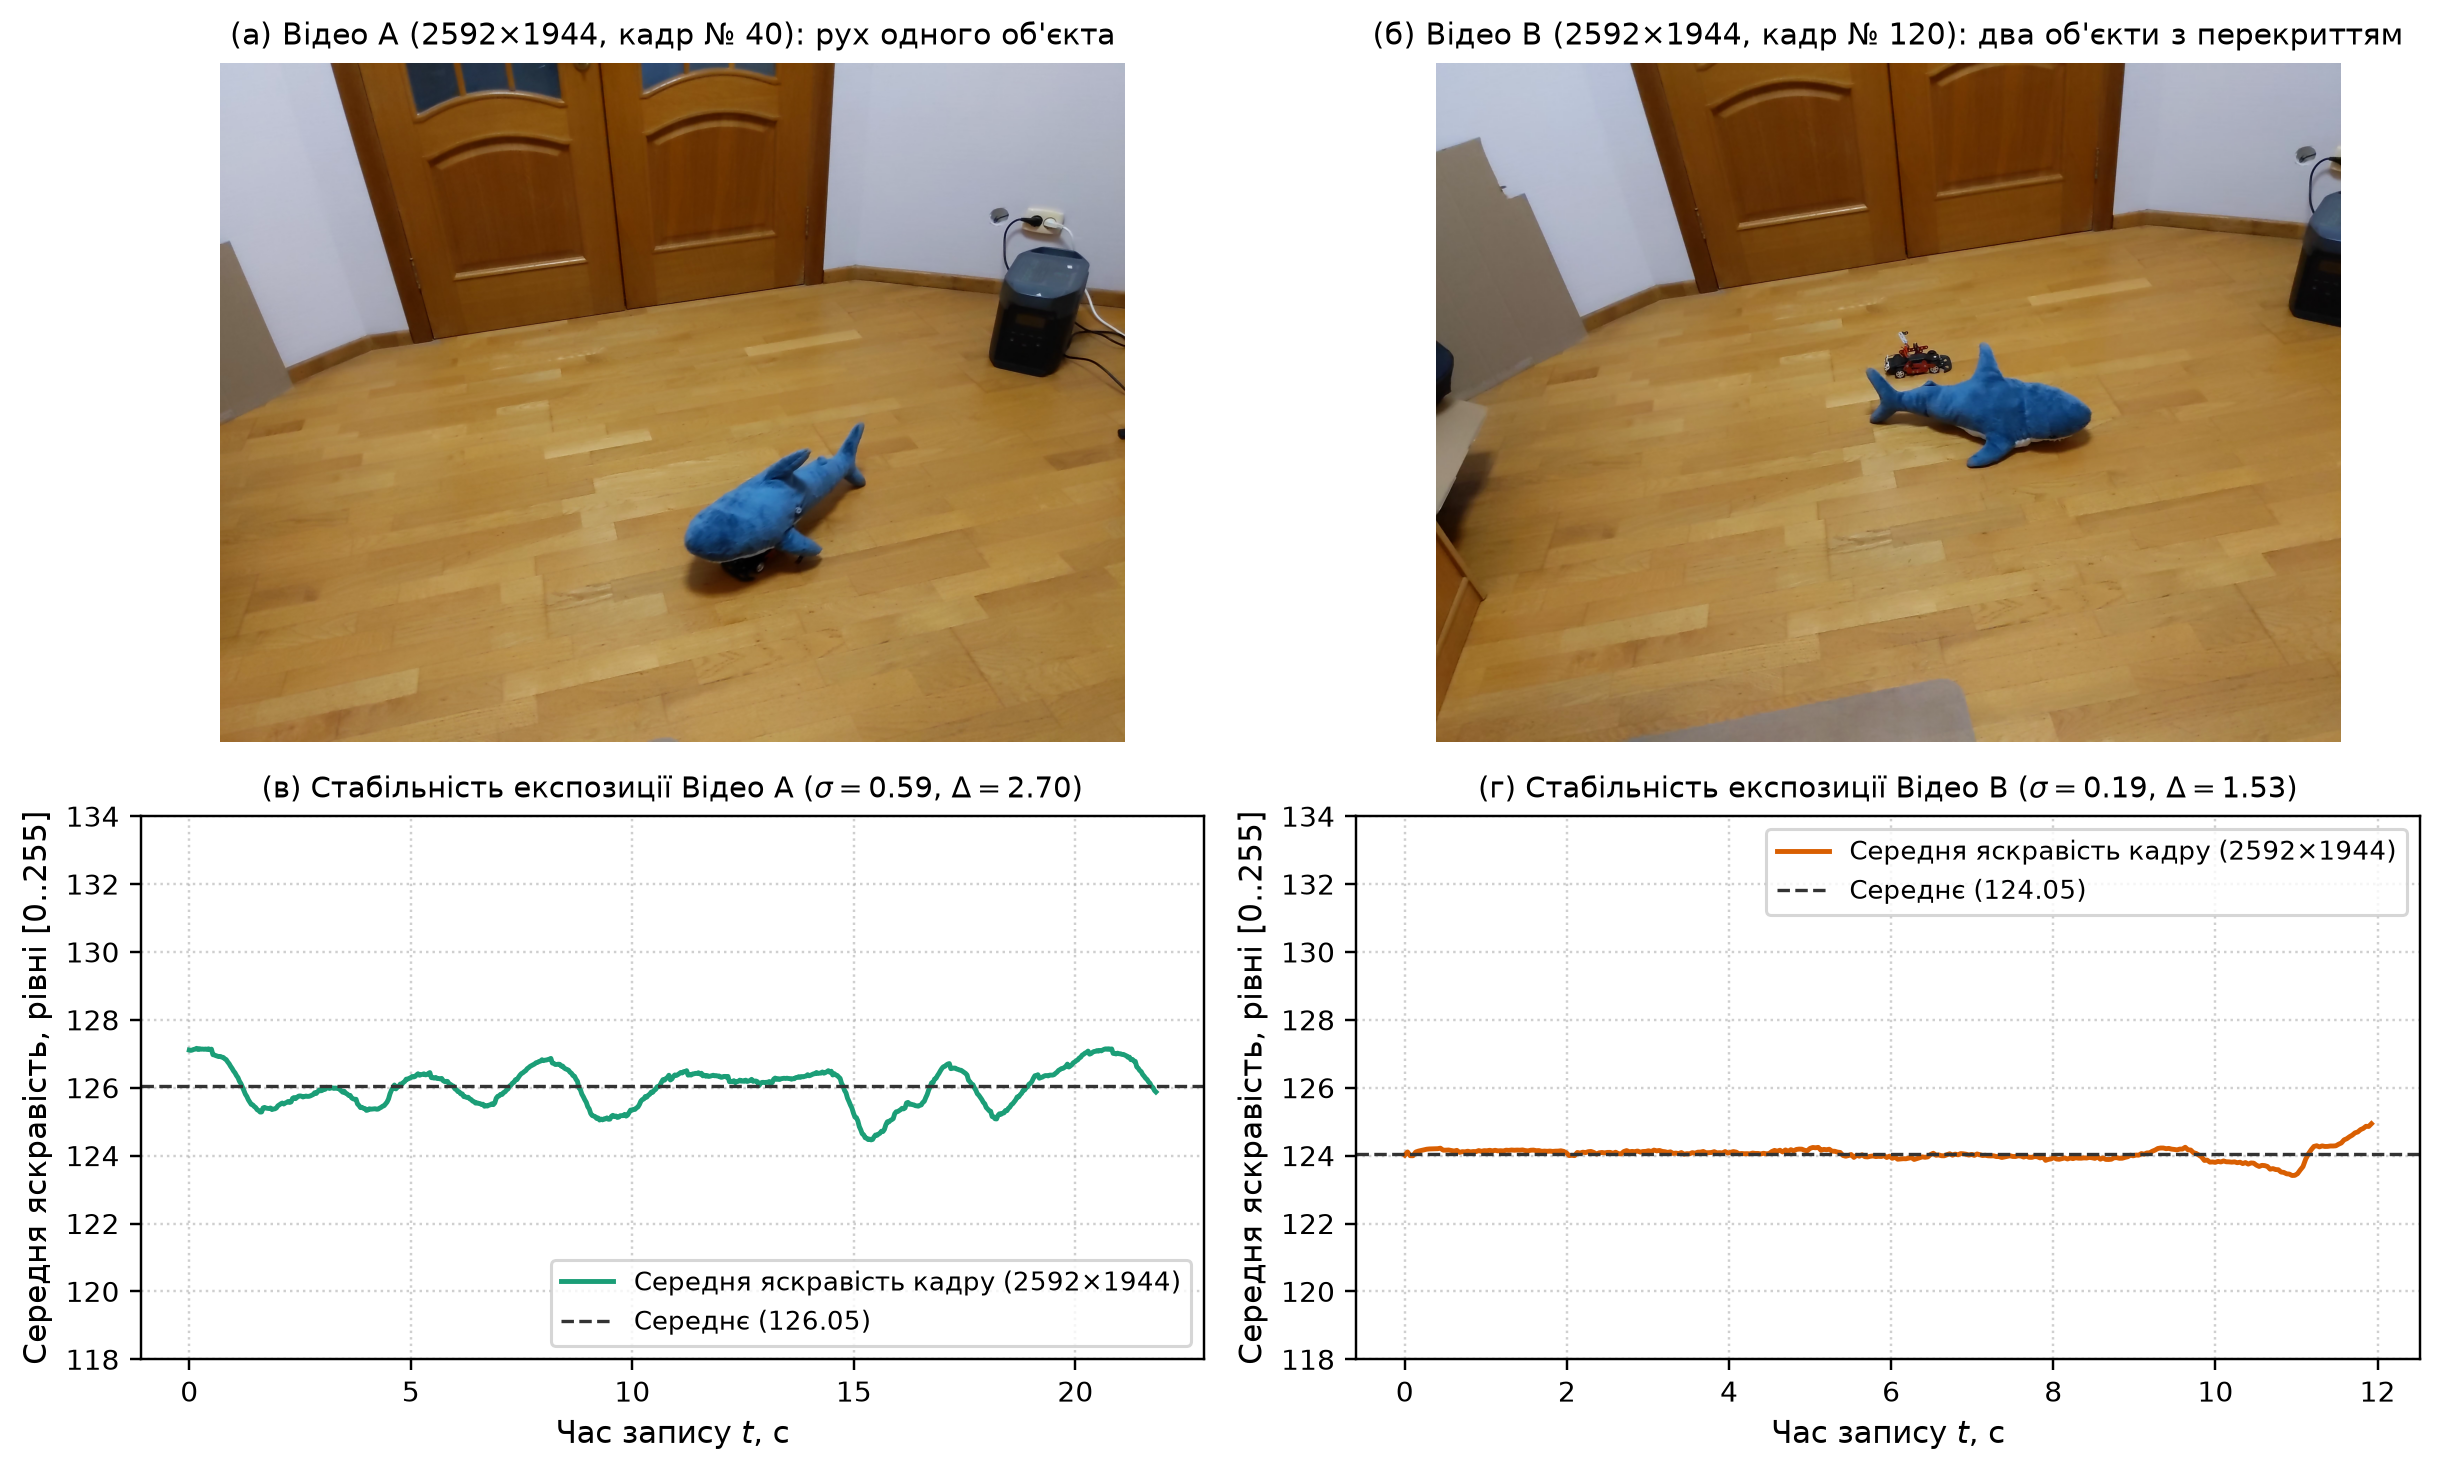
\includegraphics[width=0.98\textwidth]{../figures/a_exposure_stability.png}
    \caption{Вхідні сцени та часова стабільність середньої яскравості кадрів (Кроки 1--2): (а, б) репрезентативні кадри Відео~A та Відео~B ($2592 \times 1944$~пк); (в, г) динаміка середньої яскравості по кадрах}
    \label{fig:exposure}
\end{figure}

\begin{table}[htbp]
\centering
\caption{Виживання кутових ознак \texttt{PyrLK} без фільтрації та зі зворотною перевіркою (Частина B, Кроки 3--6)}
\label{tab:lk_summary}
\scriptsize
\setlength{\tabcolsep}{3.5pt}
\begin{tabularx}{\textwidth}{l Y c c c r}
\toprule
Відео & Режим відстеження & Усього живих & На об'єкті(ах) & На фоні & Час/кадр \\
\midrule
\directlua{tab_lk_summary()}
\bottomrule
\end{tabularx}
\end{table}

\begin{figure}[htbp]
    \centering
    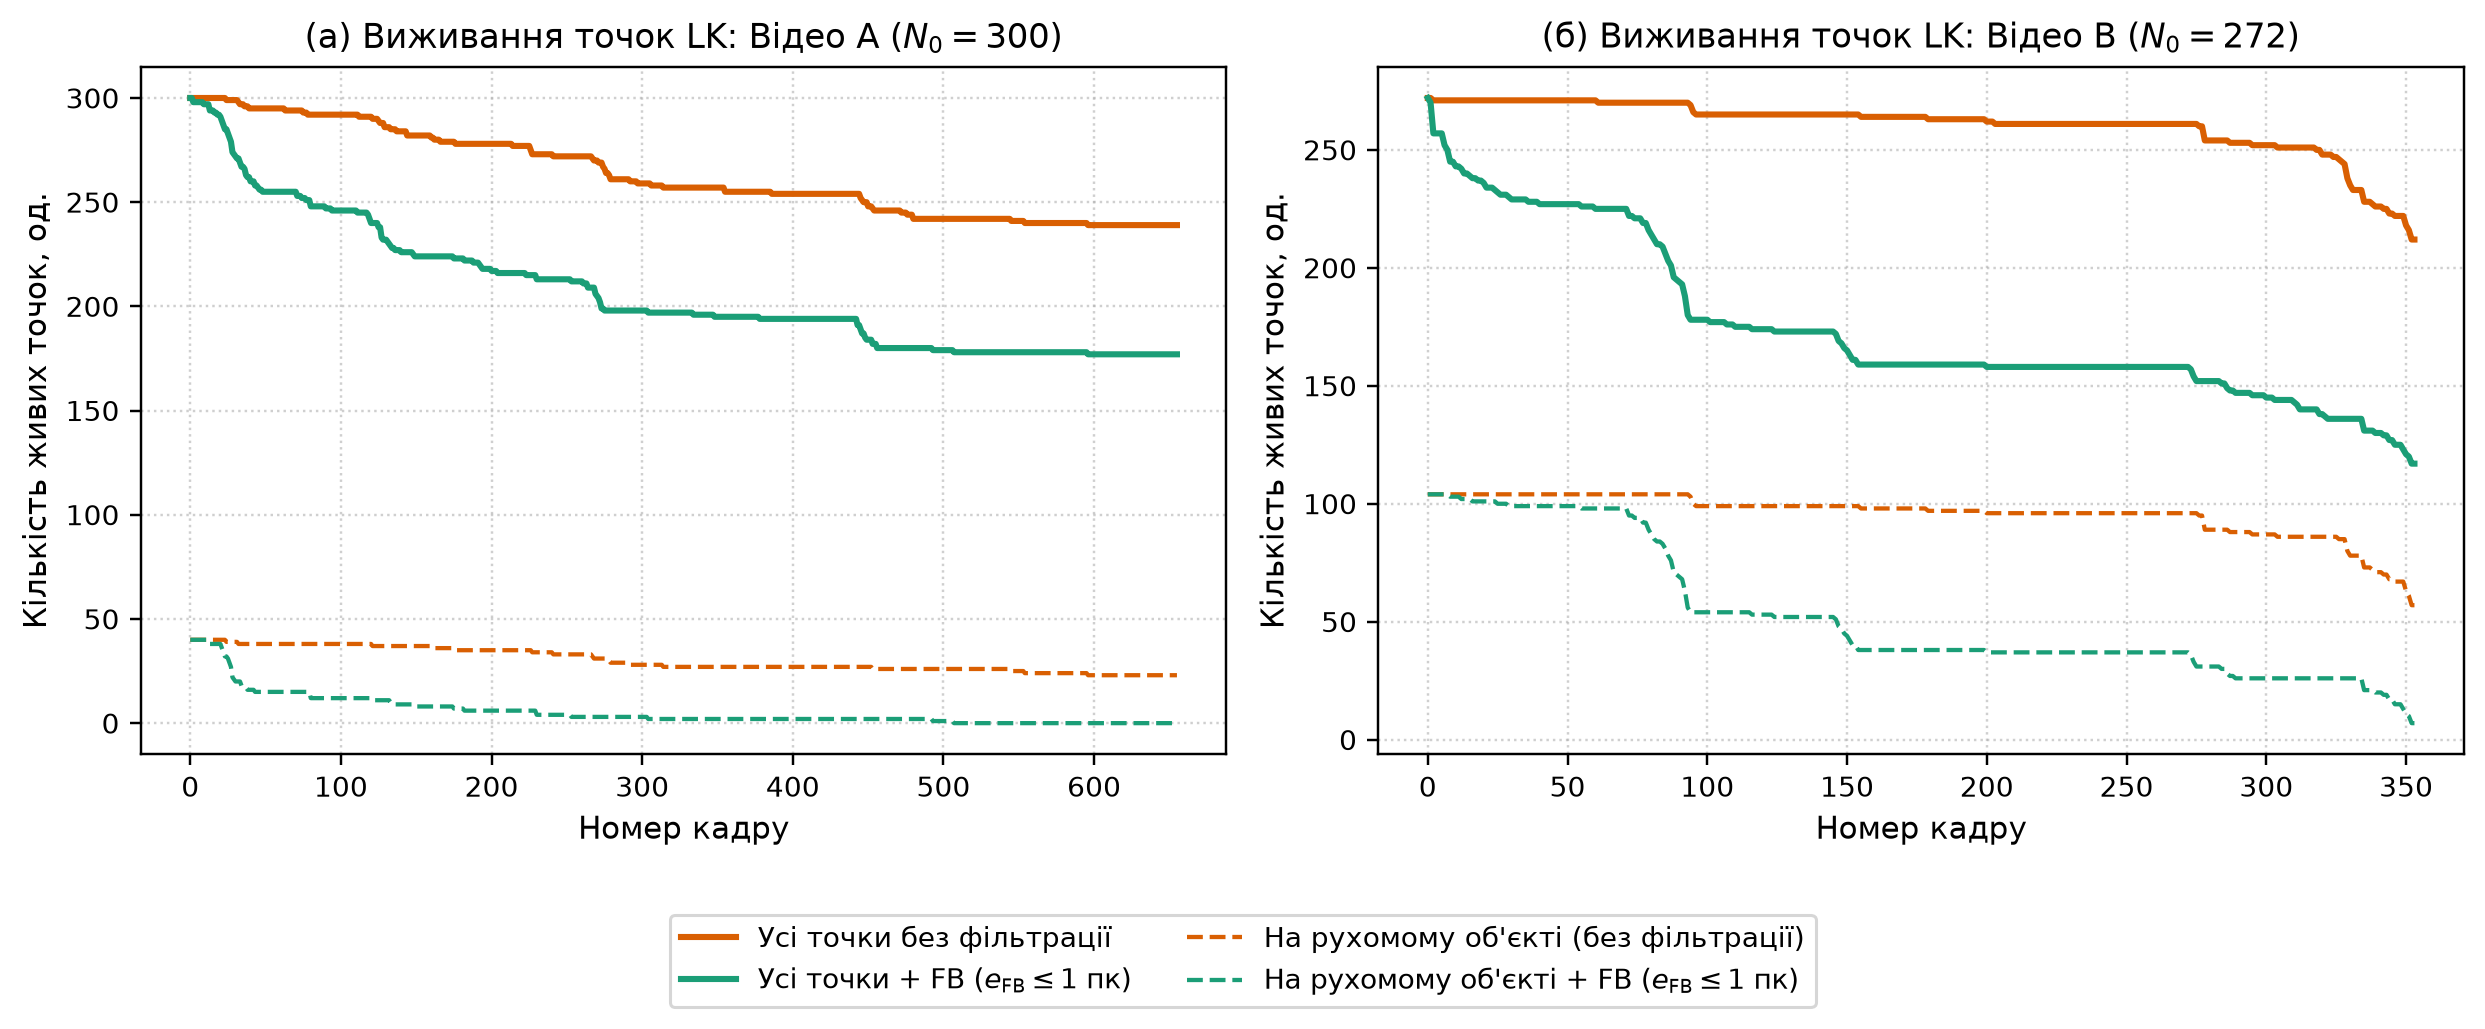
\includegraphics[width=0.98\textwidth]{../figures/b_lk_survival.png}
    \caption{Залежність кількості живих ознак Лукаса--Канаде від номера кадру без фільтрації та зі зворотною перевіркою $e_{\text{FB}} \le 1.0$~пк (Крок 6): (а) Відео~A; (б) Відео~B}
    \label{fig:lk_survival}
\end{figure}

\begin{figure}[htbp]
    \centering
    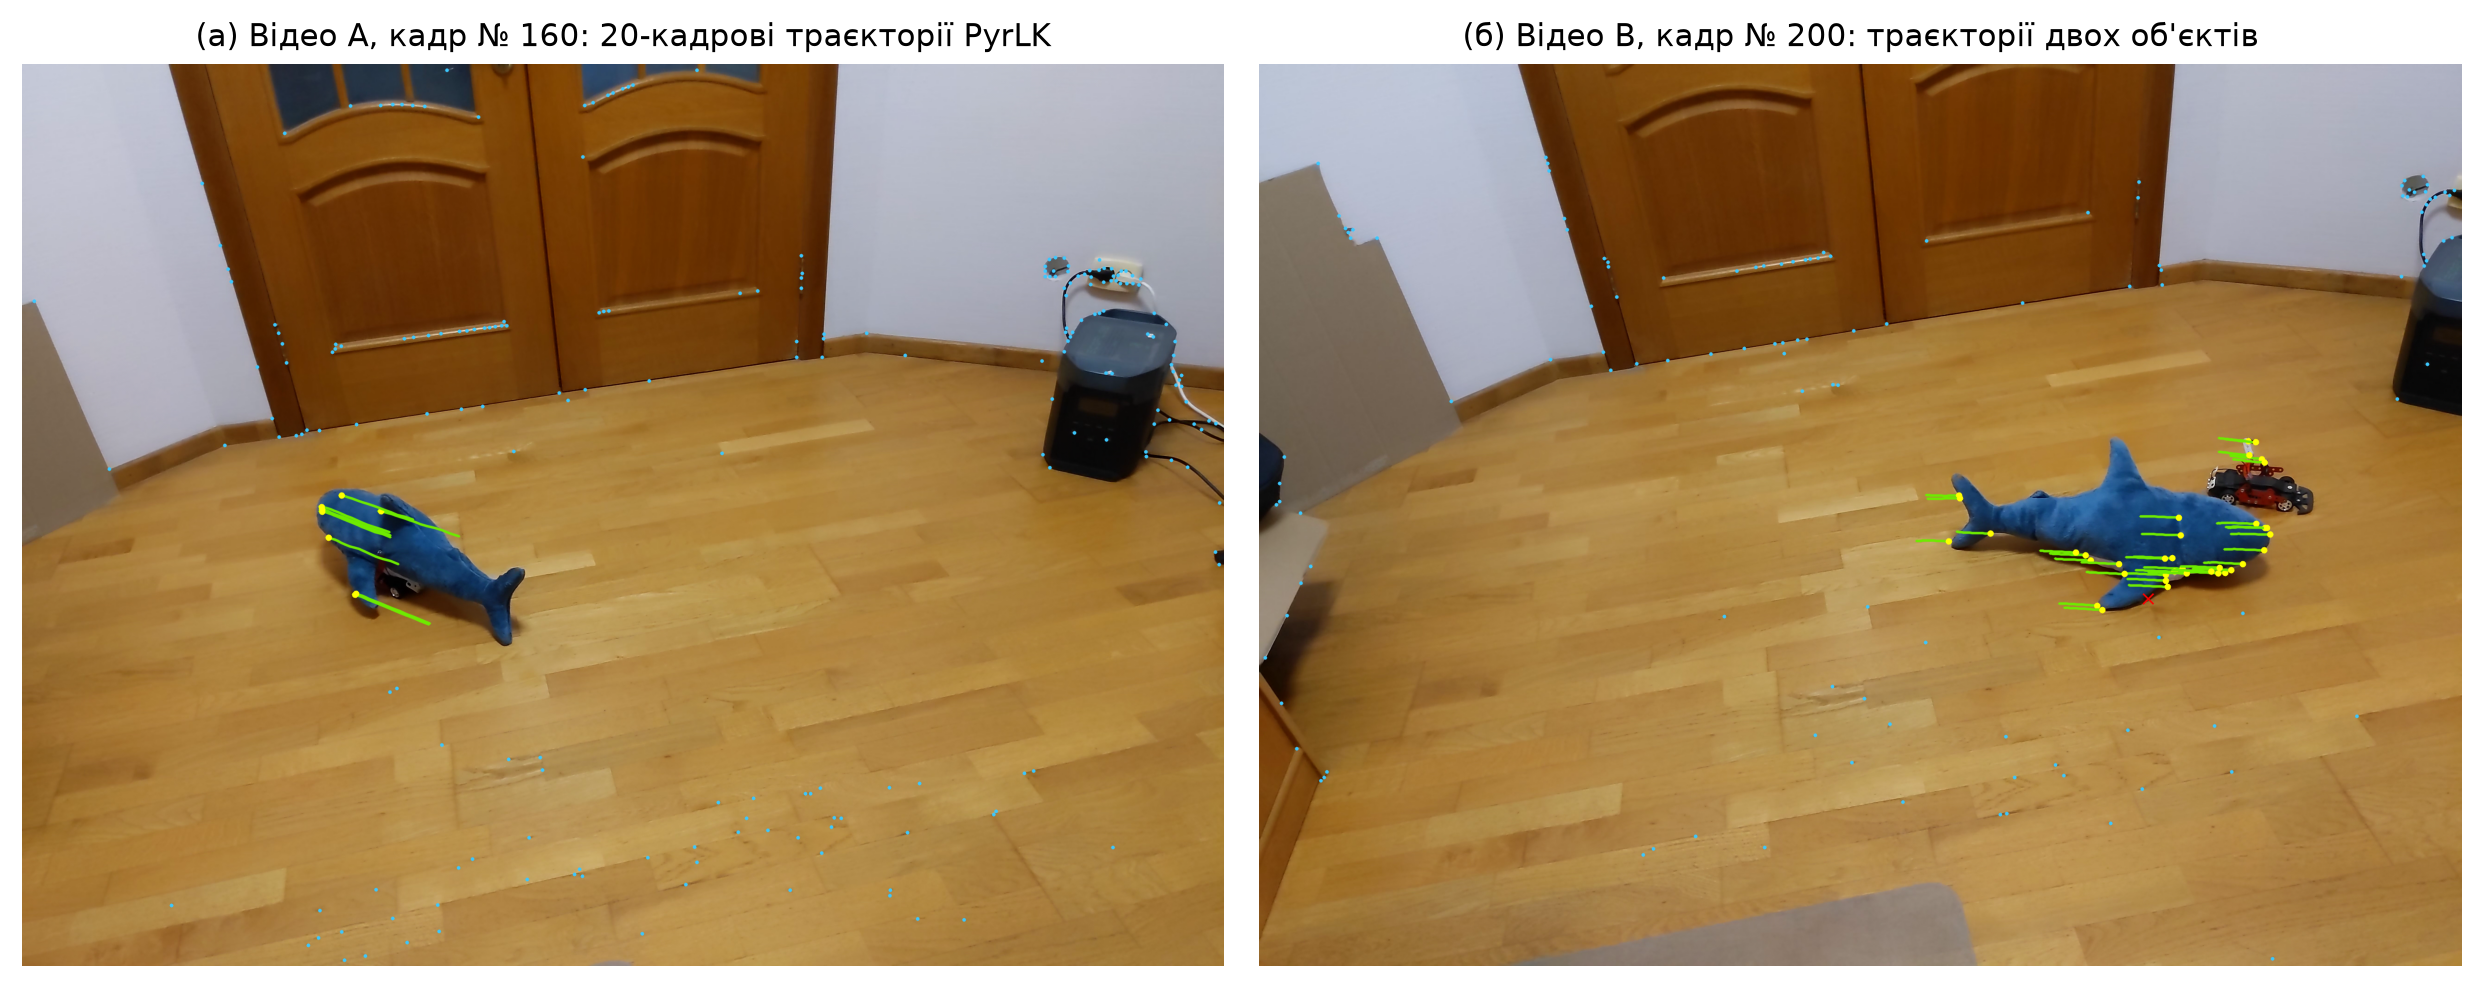
\includegraphics[width=0.98\textwidth]{../figures/b_lk_trajectories.png}
    \caption{Траєкторії останніх 20 позицій точок (зелений -- об'єкти, блакитний -- статичний фон, червоний хрестик -- відкинуті точки) (Крок 7): (а) Відео~A, кадр 160; (б) Відео~B, кадр 200}
    \label{fig:lk_trajectories}
\end{figure}

\begin{table}[htbp]
\centering
\caption{Порівняння розрідженого (\texttt{PyrLK}) і щільного (\texttt{Farneback}) оптичного потоку на $2592 \times 1944$ (Частина C, Крок 10)}
\label{tab:sparse_dense}
\scriptsize
\setlength{\tabcolsep}{3.0pt}
\begin{tabularx}{\textwidth}{>{\raggedright\arraybackslash}p{4.1cm} c r r r Y}
\toprule
Метод оптичного потоку & Роздільність & Елементи & Час $\bar{t} \pm \sigma$ & FPS & Оптимальні задачі \\
\midrule
\directlua{tab_sparse_vs_dense()}
\bottomrule
\end{tabularx}
\end{table}

\begin{figure}[htbp]
    \centering
    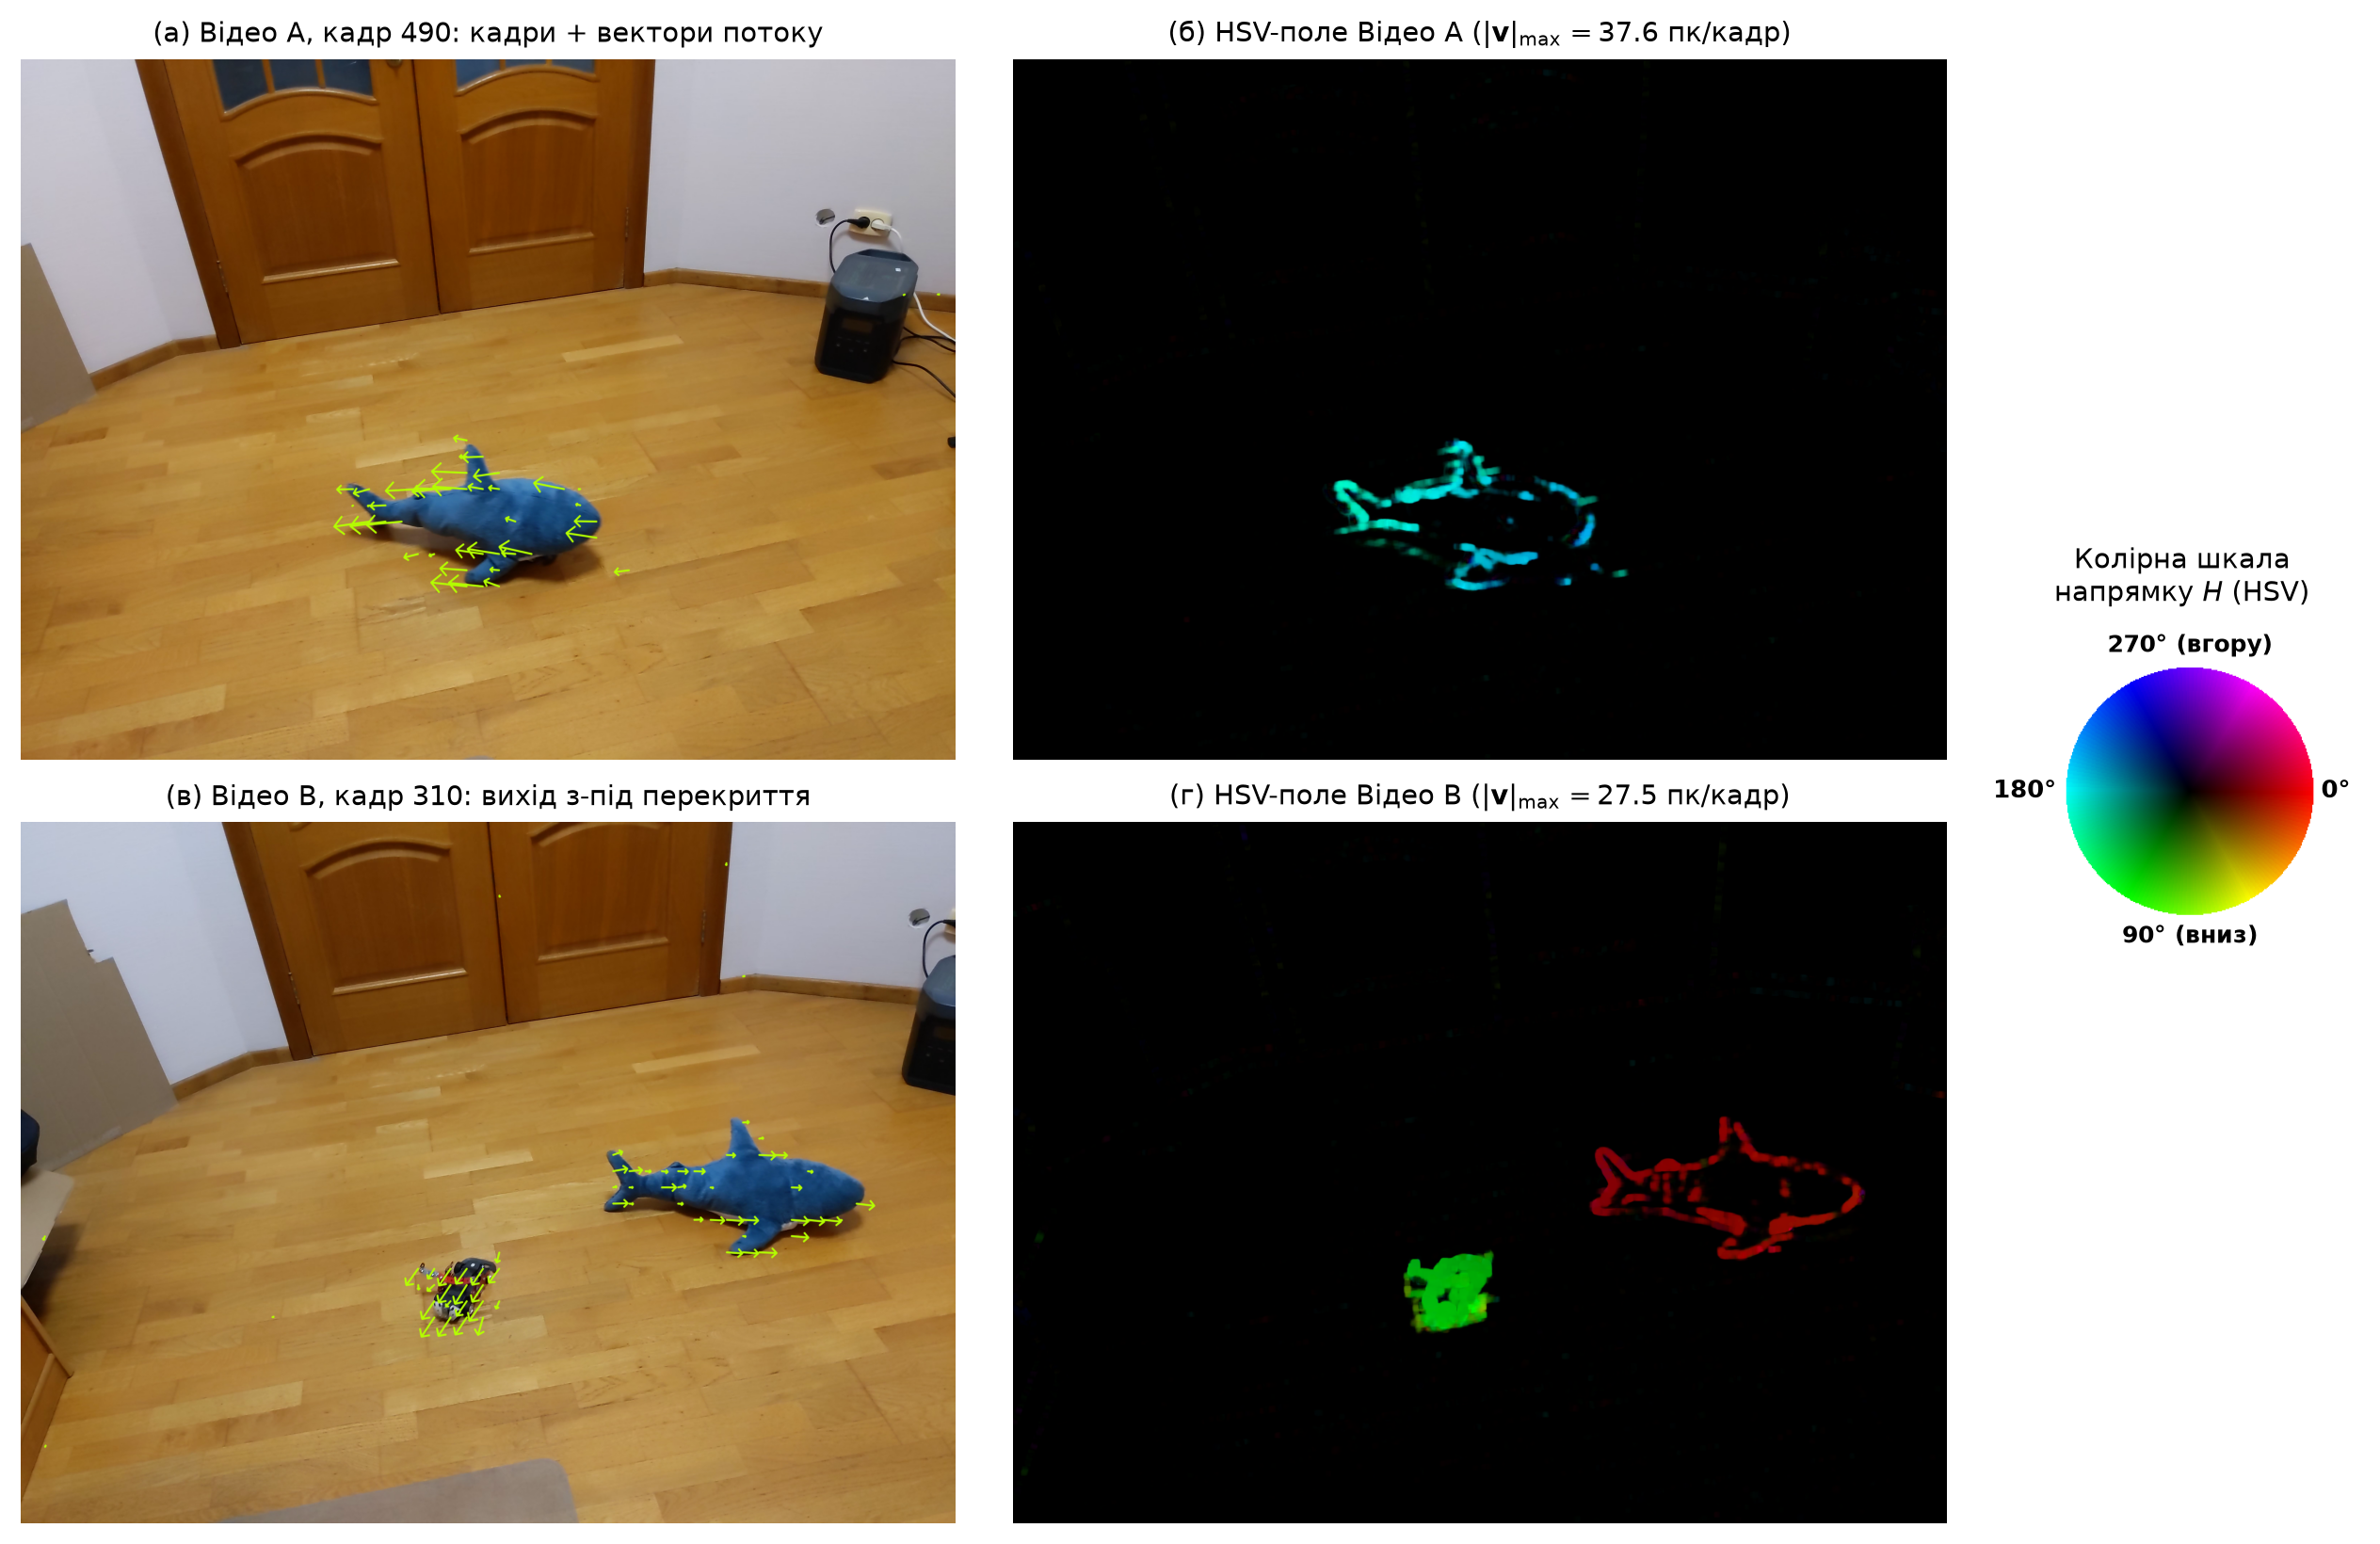
\includegraphics[width=0.98\textwidth]{../figures/c_dense_flow_hsv.png}
    \caption{Щільний оптичний потік \texttt{Farneback} та HSV-візуалізація поля швидкостей (Кроки 8--9): (а, б) Відео~A, кадр 490; (в, г) Відео~B, кадр 310; праворуч -- колірне коло напрямків $H$}
    \label{fig:dense_hsv}
\end{figure}

\begin{figure}[htbp]
    \centering
    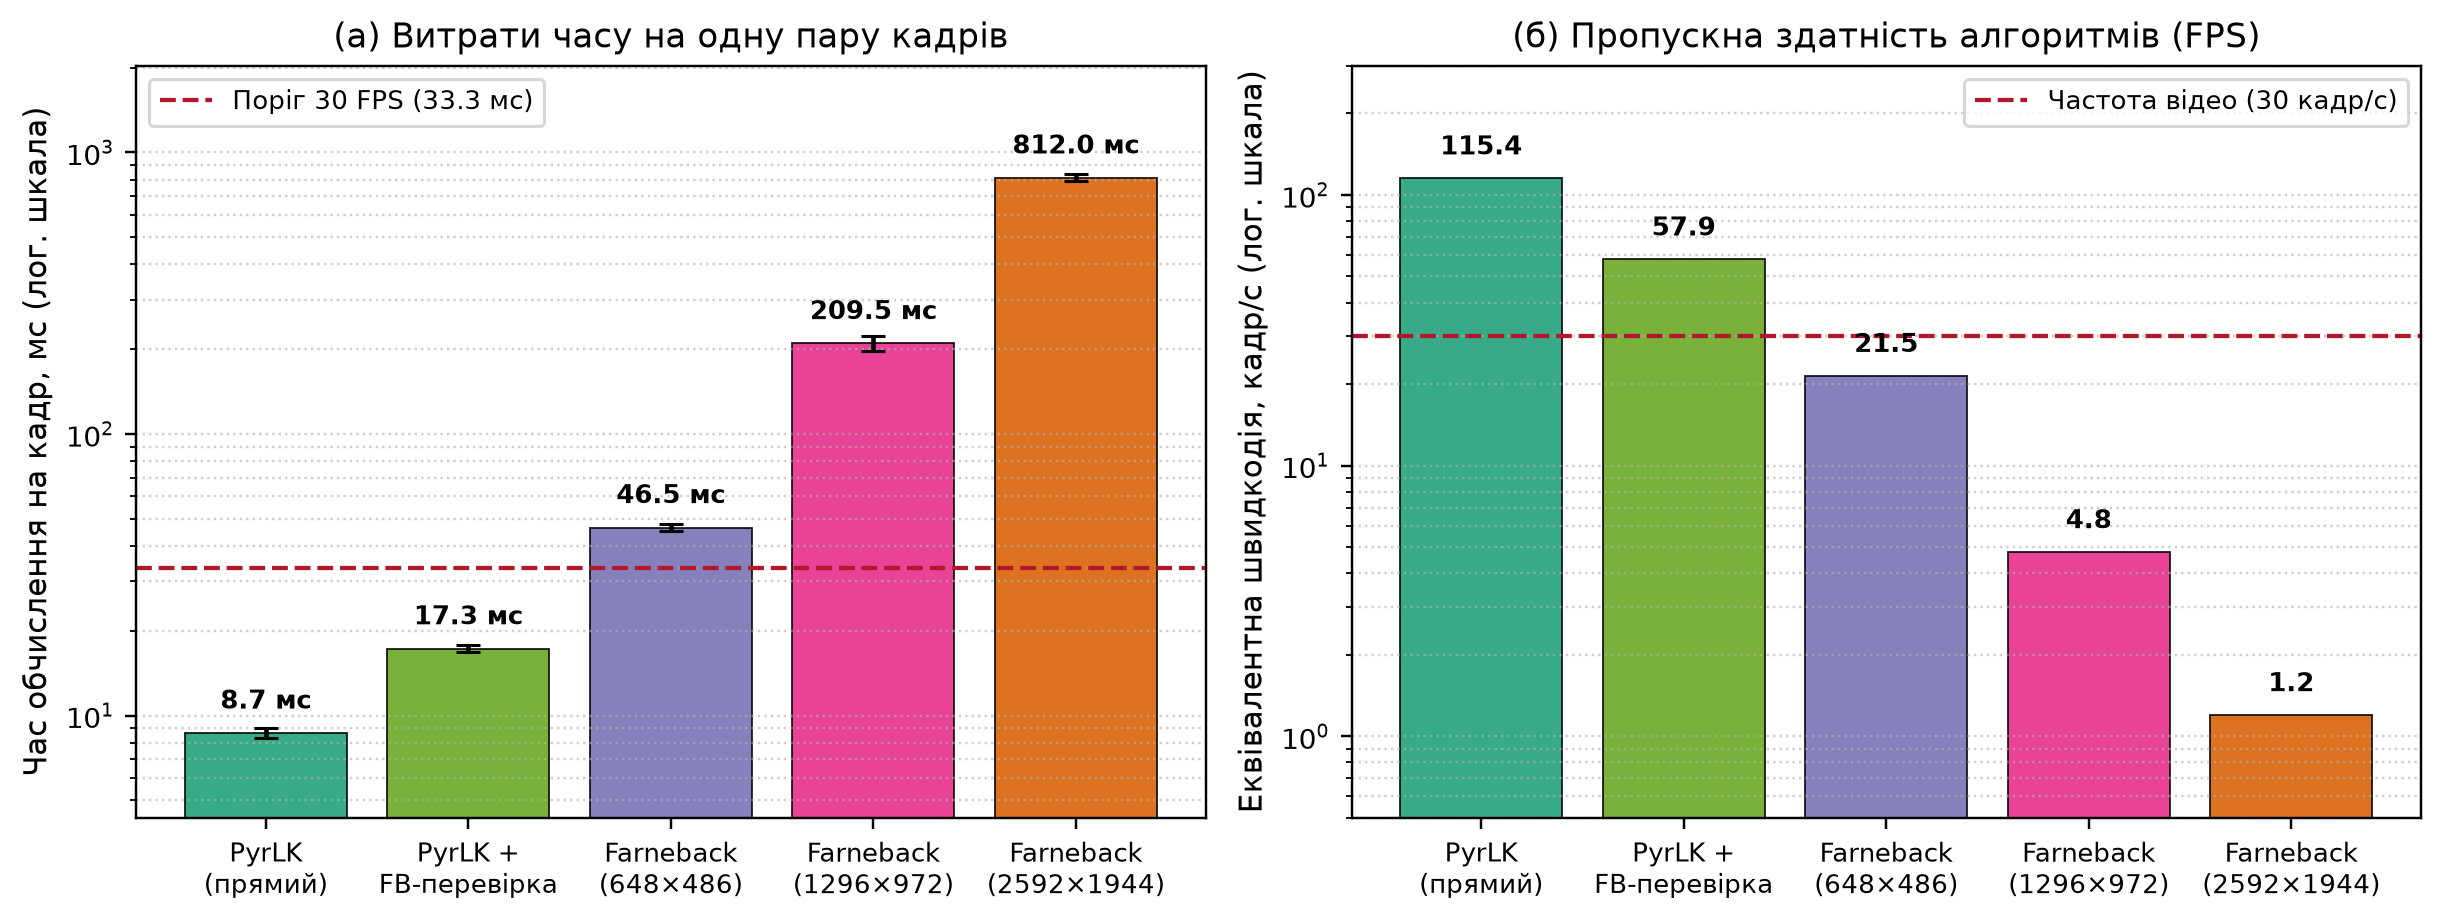
\includegraphics[width=0.98\textwidth]{../figures/c_flow_comparison.png}
    \caption{Порівняння швидкодії алгоритмів розрідженого й щільного оптичного потоку на Відео~A (Крок 10): (а) час обчислення пари кадрів (лог. шкала); (б) еквівалентна частота кадрів (FPS)}
    \label{fig:flow_comparison}
\end{figure}

\begin{table}[htbp]
\centering
\caption{Покрокове очищення маски переднього плану \texttt{MOG2} на Відео~A (Частина D, Кроки 11--13)}
\label{tab:mog2_stages}
\scriptsize
\setlength{\tabcolsep}{3.5pt}
\begin{tabularx}{\textwidth}{Y r r r c c}
\toprule
Етап конвеєра обробки & Сер. площа & Площа тіней & Частка сирої & Сер. комп./кадр & Детектовано \\
\midrule
\directlua{tab_mog2_stages()}
\bottomrule
\end{tabularx}
\end{table}

\begin{figure}[htbp]
    \centering
    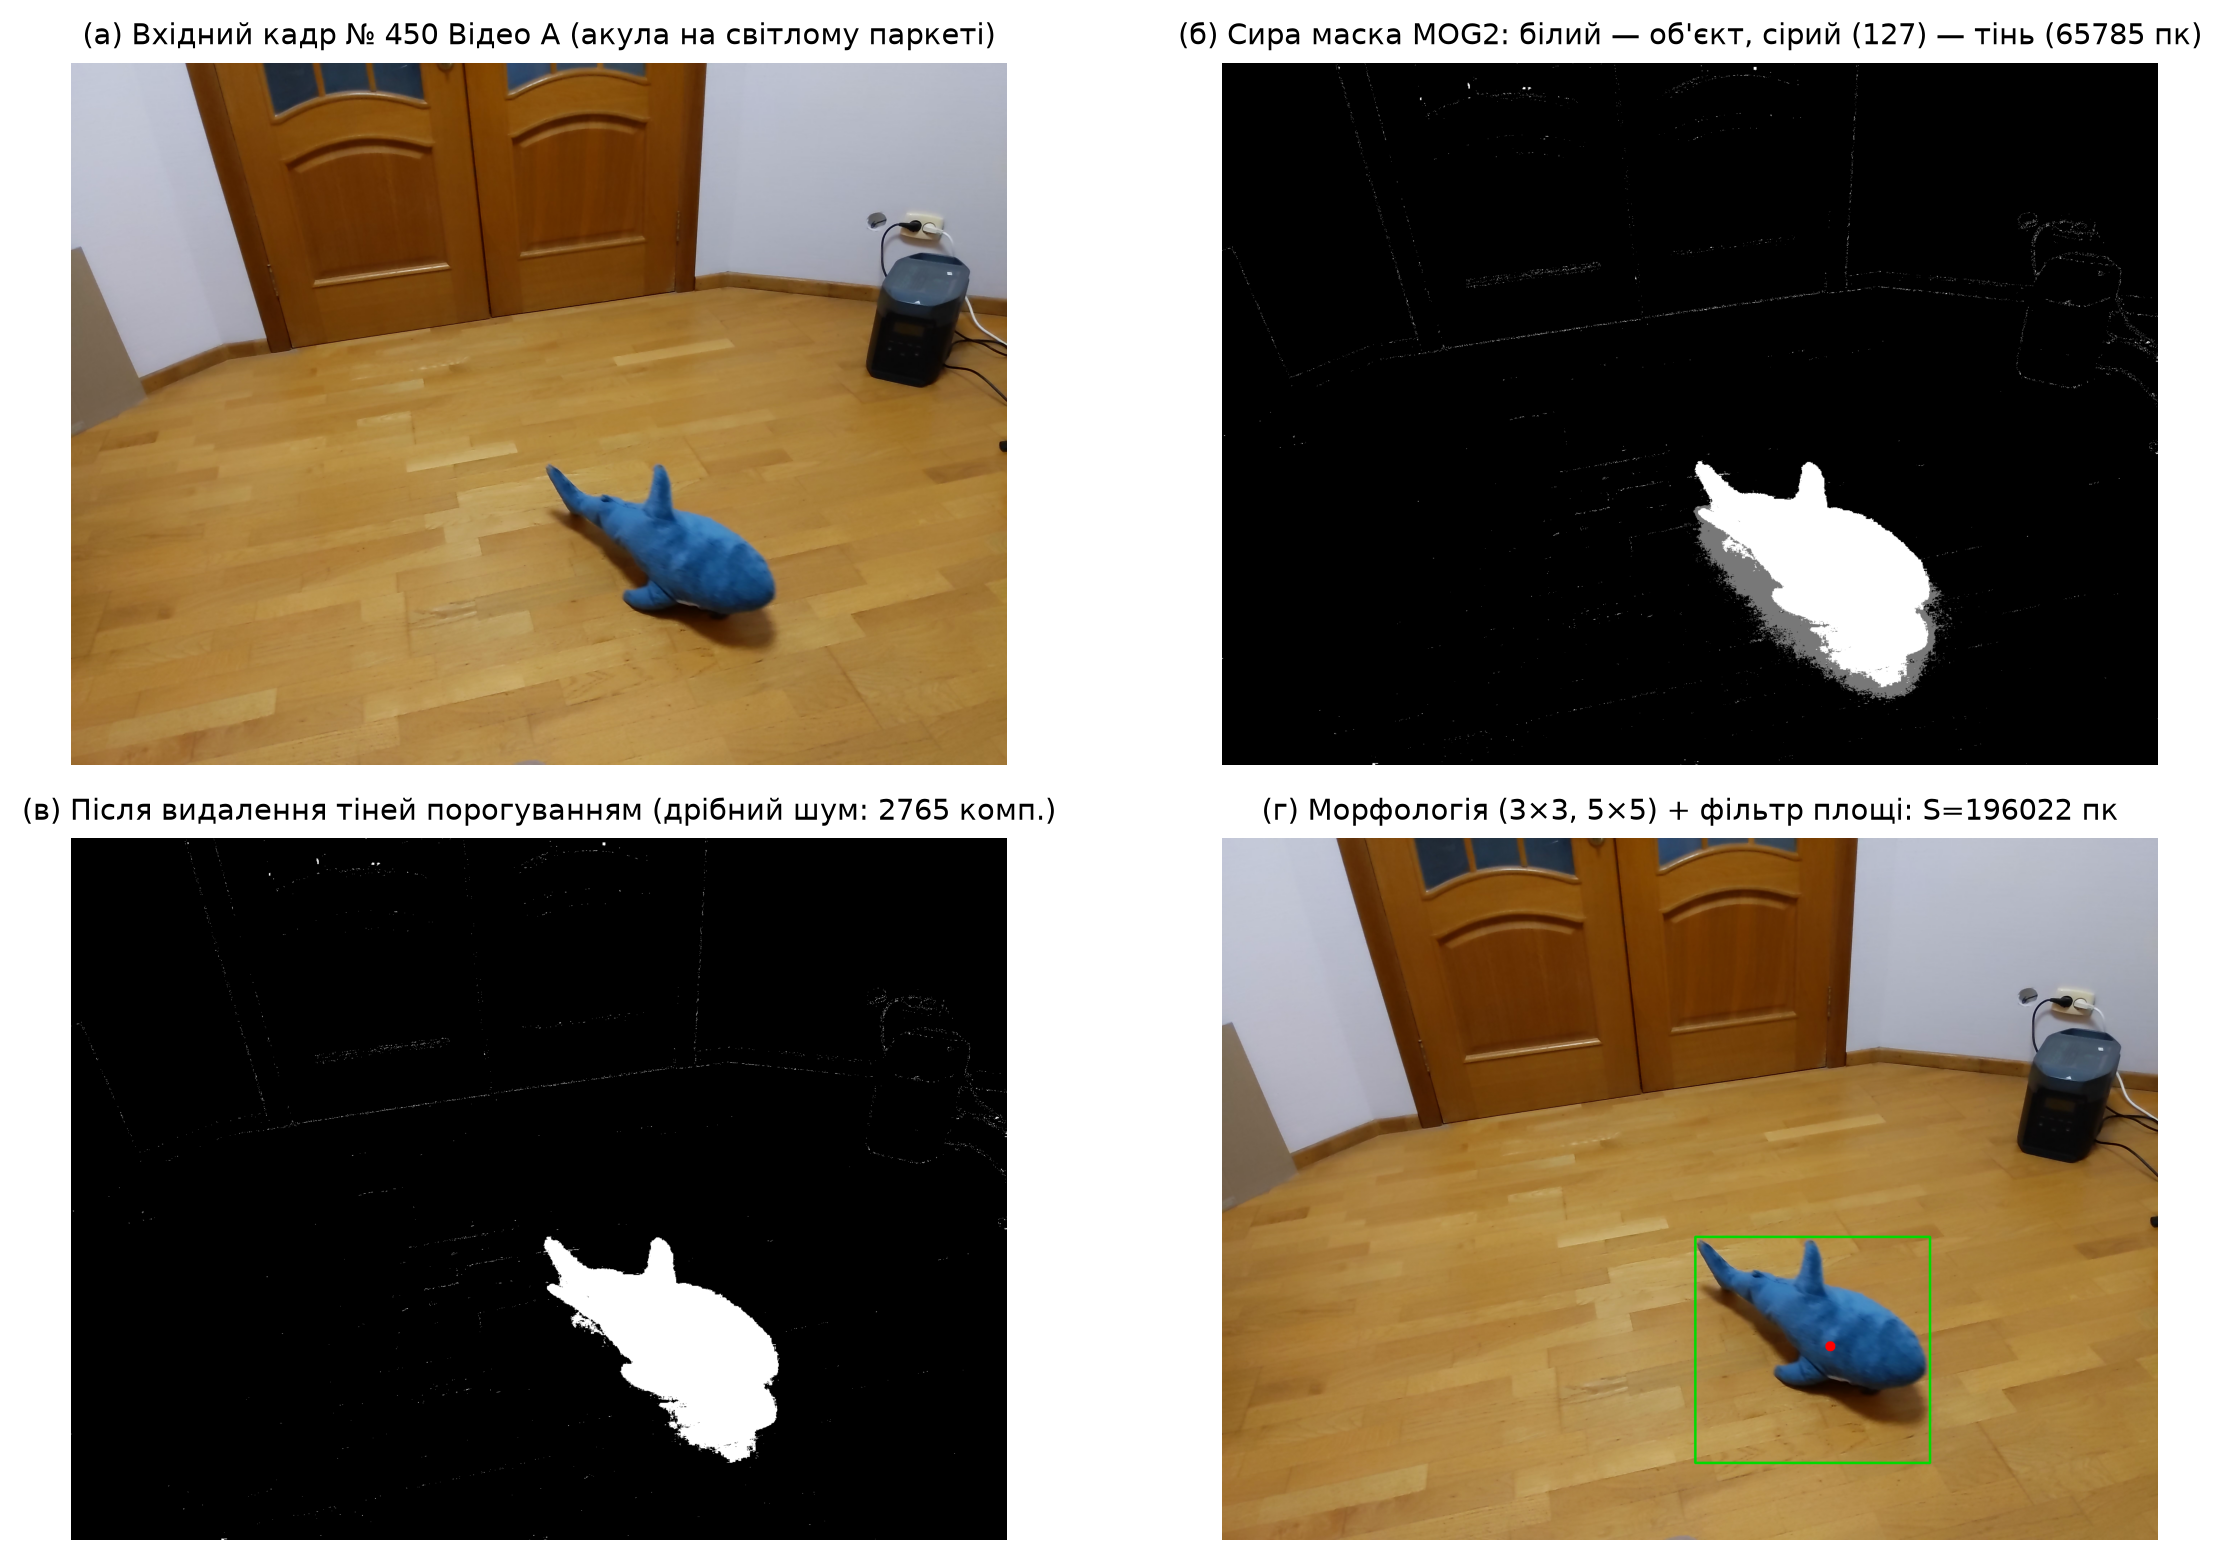
\includegraphics[width=0.98\textwidth]{../figures/d_mog2_stages.png}
    \caption{Етапи віднімання фону \texttt{MOG2} на кадрі №~450 Відео~A (Кроки 11--13): (а) вхідний кадр; (б) сира маска (\texttt{127} -- тінь); (в) видалення тіней; (г) морфологія $3{\times}3$, $5{\times}5$ та фільтр площі $S \ge 4500$~пк}
    \label{fig:mog2_stages}
\end{figure}

\begin{table}[htbp]
\centering
\caption{Точність підрахунку перетинів горизонтальної контрольної лінії у Відео~A (Частина D, Кроки 14--15)}
\label{tab:line_crossing}
\scriptsize
\setlength{\tabcolsep}{3.5pt}
\begin{tabularx}{\textwidth}{Y r r r r c r}
\toprule
Лінія $y_{\text{line}}$ & Еталон & Холодний \texttt{MOG2} & Без гістерезису & Із гістерезисом $\pm 16$~пк & Вгору / вниз & Точність \\
\midrule
\directlua{tab_line_crossing()}
\bottomrule
\end{tabularx}
\end{table}

\begin{figure}[htbp]
    \centering
    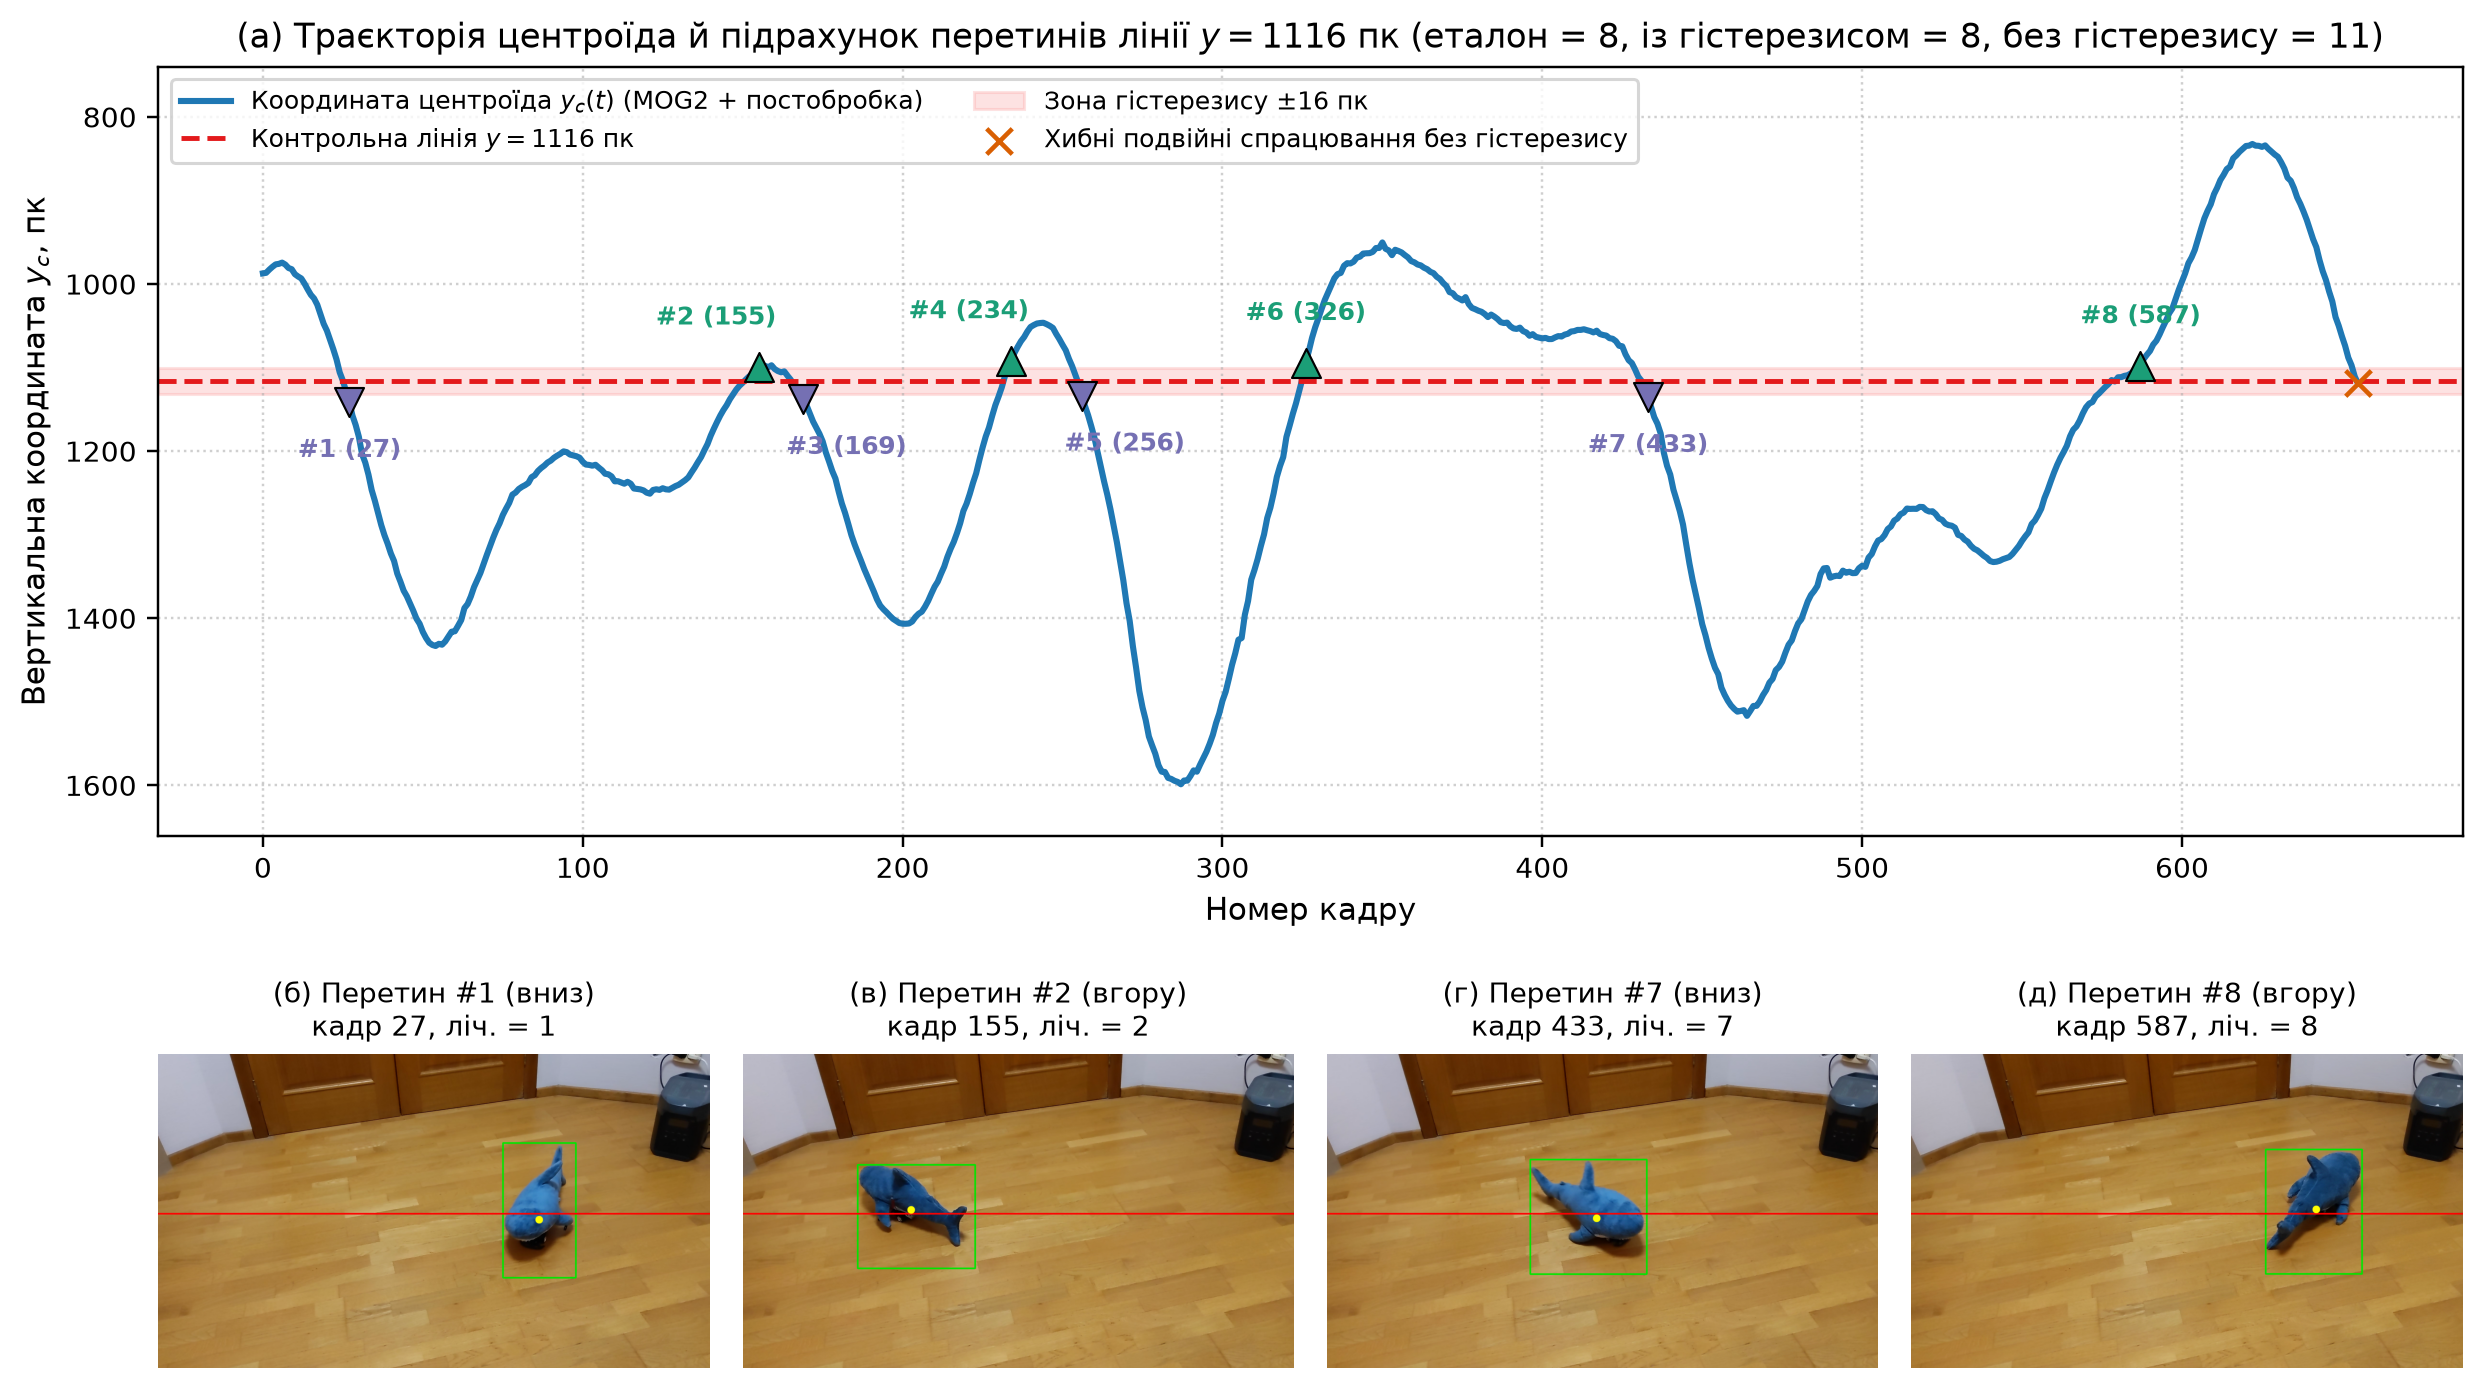
\includegraphics[width=0.98\textwidth]{../figures/d_line_crossing.png}
    \caption{Підрахунок перетинів лінії $y = 1116$~пк у Відео~A (Кроки 14--15): (а) траєкторія центроїда $y_c(t)$ із 8 впевненими перетинами та відхиленням граничного дотику на $f \approx 654$; (б--д) кадри подій лічильника}
    \label{fig:line_crossing}
\end{figure}

\begin{table}[htbp]
\centering
\caption{Кількісна оцінка надійності трекерів на 36 десятих кадрах Відео~B (Частина E, Кроки 16--19)}
\label{tab:tracking_metrics}
\scriptsize
\setlength{\tabcolsep}{3.5pt}
\begin{tabularx}{\textwidth}{Y l c c r r}
\toprule
Конфігурація трекера & Об'єкт & Утримання кадрів & Підміни ID & Сер. $e_c$ & Мед. $e_c$ \\
\midrule
\directlua{tab_tracking_metrics()}
\bottomrule
\end{tabularx}
\end{table}

\begin{figure}[htbp]
    \centering
    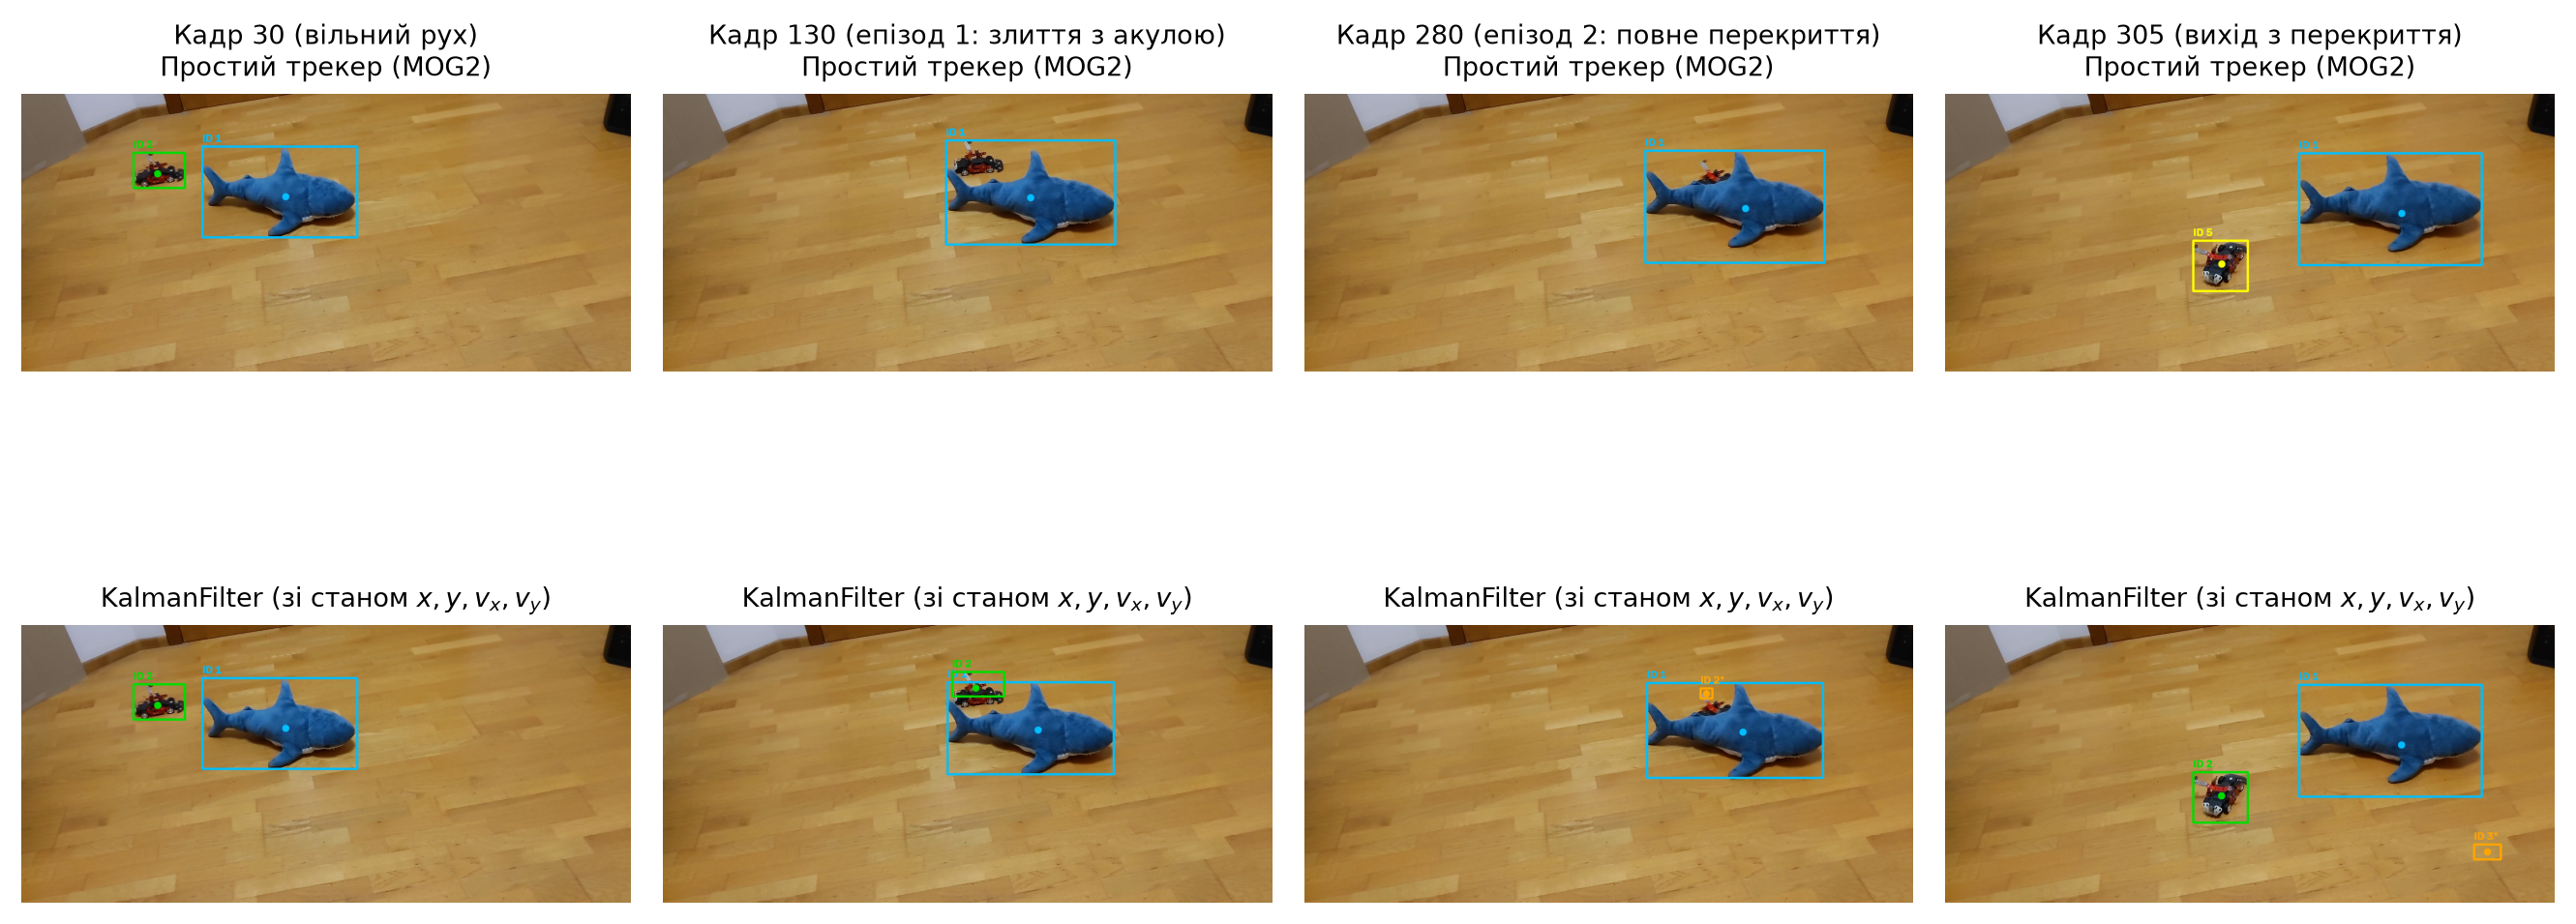
\includegraphics[width=0.98\textwidth]{../figures/e_occlusion_sequence.png}
    \caption{Порівняння простого центроїдного трекера (\texttt{MOG2}, вгорі) та \texttt{KalmanFilter(4,2)} (внизу) на ключових кадрах Відео~B: вільний рух (30), частковий дотик (130), повне перекриття (280, прогноз \texttt{ID 2*}) та вихід (305)}
    \label{fig:occlusion_seq}
\end{figure}

\begin{figure}[htbp]
    \centering
    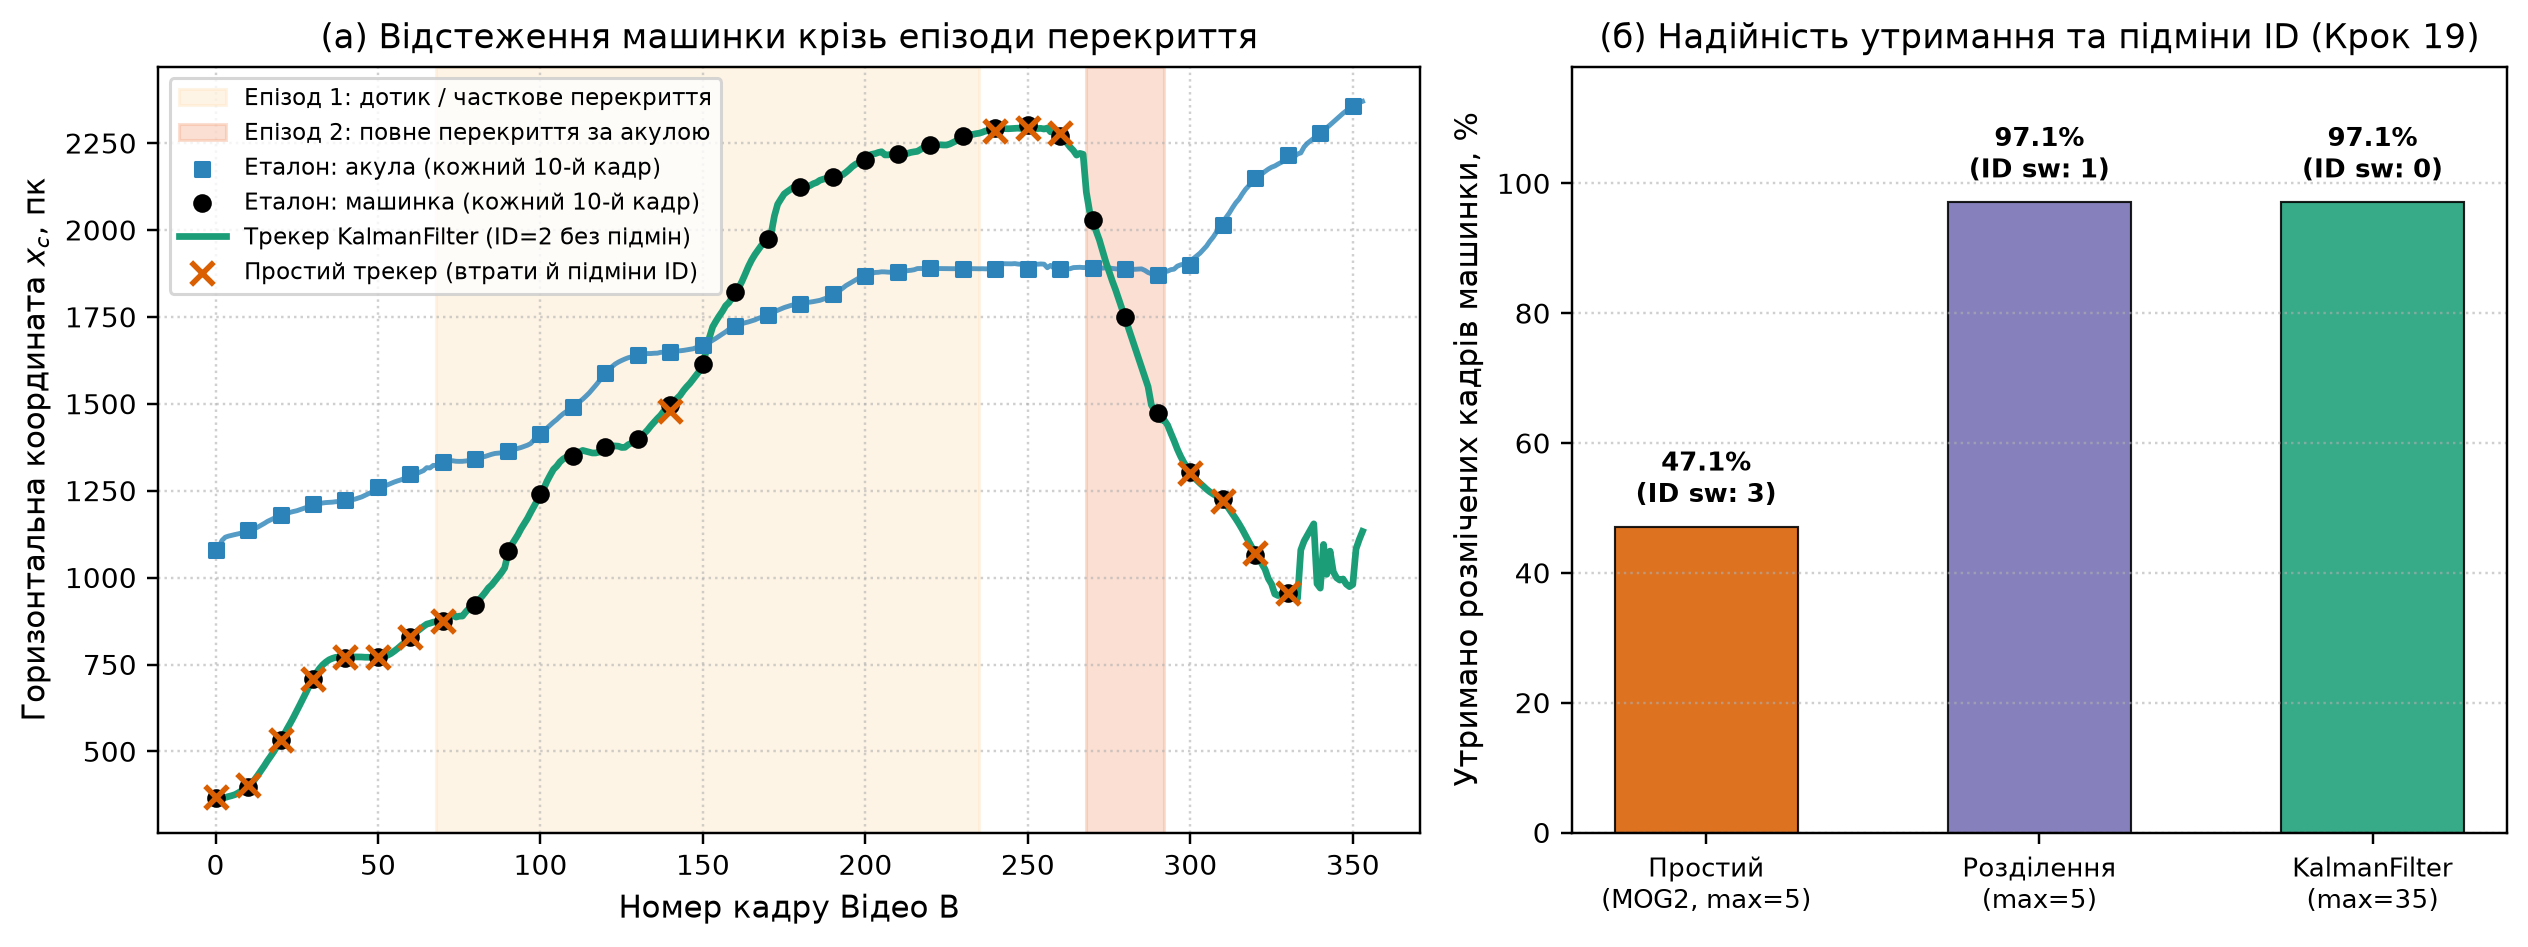
\includegraphics[width=0.98\textwidth]{../figures/e_tracking_evaluation.png}
    \caption{Кількісна оцінка відстеження машинки крізь перекриття (Кроки 18--19): (а) горизонтальна координата $x_c(t)$ відносно розмітки кожного 10-го кадру; (б) частка утриманих кадрів та підміни ID}
    \label{fig:tracking_eval}
\end{figure}

\clearpage
\section{Аналіз результатів}
\begin{enumerate}
    \item \textbf{Стабільність експозиції вхідних відео (Частина A)}: у повнокадровому форматі $2592 \times 1944$~пк середня яскравість склала $126.05 \pm 0.59$ (повний розмах $2.70$ рівнів, інтервал $124.47$--$127.16$) у Відео~A та $124.05 \pm 0.19$ (розмах $1.53$ рівнів, інтервал $123.42$--$124.94$) у Відео~B (Таблиця~\ref{tab:video_stats}, Рис.~\ref{fig:exposure}). Незначний розмах коливань ($< 1.1\%$) підтверджує зафіксовану експозицію та виконання припущення постійності яскравості~\eqref{eq:lk} без побічних бічних смуг.

    \item \textbf{Вплив зворотної перевірки \texttt{PyrLK} на рухомі та фонові ознаки (Частина B)}: у Відео~A ($300$ ознак: $40$ на акулі, $260$ на фоні) прямий потік зберігає $239/300$ ($79.7\%$) точок ($57.5\%$ на об'єкті й $83.1\%$ на фоні), а зворотна фільтрація $e_{\text{FB}} \le 1.0$~пк залишає $177/300$ ($59.0\%$): $177/260$ ($68.1\%$) на фоні й $\mathbf{0/40}$ ($\mathbf{0.0\%}$) на м'якій іграшці, оскільки тривалий рух ($21.85$~с) і розвороти руйнують текстурну симетрію вікна $21 \times 21$ (Таблиця~\ref{tab:lk_summary}, Рис.~\ref{fig:lk_survival}--\ref{fig:lk_trajectories}). У Відео~B ($272$ ознаки: $104$ на об'єктах, $168$ на фоні) прямий потік утримує $212/272$ ($77.9\%$), а зі зворотною перевіркою -- $117/272$ ($43.0\%$): $110/168$ ($65.5\%$) на фоні та лише $\mathbf{7/104}$ ($\mathbf{6.7\%}$) на рухомих об'єктах, де крива падає стрибкоподібно саме в інтервалах епізоду контакту ($f \approx 80$--$150$) та повного перекриття ($f \approx 273$--$288$).

    \item \textbf{Розріджений проти щільного потоку у високій роздільності $2592 \times 1944$ (Частина C)}: як показує бенчмарк (Таблиця~\ref{tab:sparse_dense}, Рис.~\ref{fig:flow_comparison}), розріджений \texttt{PyrLK} для $300$ ознак навіть на $5$-мегапіксельному кадрі ($2592 \times 1944$) працює швидше реального часу: $\mathbf{8.67 \pm 0.33}$~мс/кадр ($\mathbf{115.4}$~FPS) у прямому проході та $\mathbf{17.27 \pm 0.47}$~мс ($\mathbf{57.9}$~FPS) зі зворотною перевіркою. Повнокадровий щільний \texttt{Farneback} ($5\,038\,848$ пікселів) вимагає $\mathbf{811.96 \pm 22.61}$~мс ($\mathbf{1.2}$~FPS), що у $\mathbf{93.7}$ раза повільніше за прямий \texttt{PyrLK}. Зменшення масштабу до $0.25\times$ ($648 \times 486$) прискорює \texttt{Farneback} у $17.5$ раза (до $46.52$~мс, $21.5$~FPS). Попри високу обчислювальну вартість, щільне HSV-поле (Рис.~\ref{fig:dense_hsv}) чітко розділяє напрямки руху при розходженні об'єктів: на кадрі 310 Відео~B акула праворуч зафарбована червоним ($0^\circ$), а машинка вниз-ліворуч -- зеленим ($90^\circ$--$135^\circ$) без жодного числового викиду нормування.

    \item \textbf{Очищення \texttt{MOG2} і чутливість гістерезису на перетинах (Частина D)}: на $2592 \times 1944$ маска \texttt{MOG2} виділяє об'єкт разом із тінню ($211\,343$~пк, із них $\mathbf{42\,378}$~пк тіні \texttt{127}, або $20.1\%$; Таблиця~\ref{tab:mog2_stages}, Рис.~\ref{fig:mog2_stages}). Відсікання тіней ($\texttt{raw} > 200$) залишає $4451.7$ дрібних шумових компонент на кадр; морфологія $3{\times}3$, $5{\times}5$ та фільтр площі $S \ge 4500$~пк доводять кількість компонент до $\mathbf{1.12}$/кадр із детекцією у $\mathbf{656/656}$ ($100\%$) кадрів (проти $643/656$ при холодному старті). У тесті перетинів контрольної лінії (Таблиця~\ref{tab:line_crossing}, Рис.~\ref{fig:line_crossing}):
    \begin{itemize}
        \item холодний старт \texttt{MOG2} генерує $10$--$13$ перетинів (при еталоні $8$) через нестабільність маски на старті запису;
        \item на висоті $y = 1116$~пк без гістерезису фіксується $11$ перетинів (додаткові хибні спрацювання на повороті та на фініші на межі лінії біля кадру $654$), тоді як зона гістерезису $\pm 16$~пк пропускає неглибоке наближення до $y \approx 1096$~пк на кадрі $155$ ($20 > 16$~пк) й відсікає граничний торк на кадрі $654$, даючи точні $\mathbf{8/8}$ ($\mathbf{100.0\%}$: $4$ вгору та $4$ вниз);
        \item на лінії $\mathbf{y = 1152}$~пк алгоритм також досягає $\mathbf{100.0\%}$ ($\mathbf{8/8}$), а на $y = 1100$~пк -- $7/8$ ($87.5\%$) проти $9$ без гістерезису.
    \end{itemize}

    \item \textbf{Порівняння трекерів крізь перекриття у Відео~B (Частина E)}: на $34$ розмічених десятих кадрах присутності машинки ($0..330$) у Відео~B відбувається тривале часткове накладання контурів ($f = 68$--$235$) та повне перекриття ($f = 273$--$288$, $16$ кадрів; Таблиця~\ref{tab:tracking_metrics}, Рис.~\ref{fig:occlusion_seq}--\ref{fig:tracking_eval}):
    \begin{itemize}
        \item \textit{Трекер 1 (простий центроїдний на масках \texttt{MOG2}, $\texttt{max\_lost} = 5$)}: через злиття масок похибка центру акули зростає до $34.3$~пк, а трек машинки втрачається на обох перекриттях -- утримано лише $\mathbf{16/34 = 47.1\%}$ кадрів із \textbf{$\mathbf{3}$ підмінами ID} (\texttt{ID 2 -> 3 -> 4 -> 5});
        \item \textit{Трекер 2 (центроїдний + розділення силуетів, $\texttt{max\_lost} = 5$)}: бездоганно супроводжує обидва об'єкти протягом епізоду 1 ($68$--$235$, піднімаючи утримання до $\mathbf{33/34 = 97.1\%}$ та знижуючи середню похибку по акулі в $3.8$ раза -- з $34.3$ до $9.0$~пк), однак не переживає $16$-кадрове повне перекриття $273$--$288$ ($> 5$ кадрів) і перереєстровує машинку як \texttt{ID 4} (\textbf{$\mathbf{1}$ підміна ID});
        \item \textit{Трекер 3 (\texttt{cv2.KalmanFilter(4,2)} + розділення, $\texttt{max\_lost} = 35$)}: прогнозує траєкторію машинки крізь усе повне перекриття за оціненим вектором швидкості $(v_x, v_y)^T$, з похибкою лише $4.7$~пк підхоплює вихід машинки на кадрі $290$ ($x = 1469.9$ проти еталона $1473.1$~пк) та утримує виключно \texttt{ID 2} на всій дистанції до $f=330$ (\textbf{$\mathbf{0}$ підмін ID}, медіанна похибка $\mathbf{3.2}$~пк, утримання $\mathbf{33/34 = 97.1\%}$ через те, що на прихованому кадрі $280$ прогноз іде дещо вище інтерпольованого центру мас за видимим дахом машинки).
    \end{itemize}
\end{enumerate}

\section{Висновки}
\begin{enumerate}
    \item Перевірено нові повнокадрові відеопослідовності $2592 \times 1944$~пк ($656$ кадрів Відео~A та $354$ кадри Відео~B) без бічних смуг: доведено високу стабільність експозиції (розмах $\le 2.70$ рівнів сірого).
    \item Показано, що зворотна перевірка \texttt{PyrLK} ($e_{\text{FB}} \le 1.0$~пк) ефективно відсіває дрейф точок при поворотах і перекриттях (на рухомих об'єктах виживає $0.0\%$--$6.7\%$ проти $65.5\%$--$68.1\%$ на статичному фоні), а розріджений \texttt{PyrLK} на $2592 \times 1944$ працює у реальному часі ($8.67$~мс, $115.4$~FPS) і у $\mathbf{93.7}$ раза швидше за повнокадровий щільний \texttt{Farneback} ($811.96$~мс, $1.2$~FPS).
    \item Конвеєр \texttt{MOG2} із відсіканням тіней (\texttt{127}), морфологією $3{\times}3 / 5{\times}5$ та фільтром площі $S \ge 4500$~пк забезпечує детекцію об'єкта на $100\%$ кадрів ($656/656$), а підрахунок перетинів із гістерезисом $\pm 16$~пк досягає $100.0\%$ точності ($8/8$) як на $y = 1116$~пк, так і на $y = 1152$~пк (проти $11$ без гістерезису і $12$ на холодному старті).
    \item На $36$ розмічених десятих кадрах Відео~B підтверджено, що поєднання розділення силуетів і фільтра Калмана \texttt{cv2.KalmanFilter(4, 2)} знижує кількість підмін ID машинки через перекриття з $3$ (простий трекер, $47.1\%$ утримання) та $1$ (розділення без Калмана) до \textbf{$\mathbf{0}$ підмін} за медіанної похибки супроводу $3.2$~пк та утримання $97.1\%$ ($33/34$).
\end{enumerate}

\section{Декларація про використання генеративного ШІ}
Під час виконання даної лабораторної роботи генеративний штучний інтелект (агентська система Antigravity) використовувався як інструмент парного програмування для автоматизації написання скриптів обчислювальних експериментів з оптичного потоку, віднімання фону \texttt{MOG2} та фільтрації Калмана, формування візуалізацій і верстки звіту в середовищі LuaLaTeX відповідно до ДСТУ 3008:2015. Усі відеодані, алгоритми, критерії оцінювання та інтерпретації кількісних результатів перевірено автором.

\end{document}
